%Definiciones previas y uso de paqueterías
\documentclass[12pt]{article}
\usepackage[utf8]{inputenc}
\usepackage{graphicx} % Required for inserting images
\usepackage[spanish]{babel}
\usepackage{geometry}
\usepackage{setspace}
\usepackage{sectsty} %Para cambiar el tamaño de diferentes secciones

%Para el formato APA
\usepackage{apacite}

%Márgenes
\newgeometry{left=1in, right=1in, top=1in, bottom=1in}

\begin{document}

%Haciendo portada
\begin{titlepage}
\centering
{
\includegraphics[width=0.40\textwidth]{imagenes/1 escudo san marcos.png}\par}
\vspace{0.5cm}
{\bfseries\Large Universidad Nacional Mayor de San Marcos\par}
{\large Universidad del Perú, Decana de América\par}
{\scshape\Large Facultad de Ingeniería de Sistemas e Informatica\par}
{\scshape\Large Escuela Profesional de Ingeniería de Sistemas\par}
\vspace{0.5cm}
{\bfseries\large Informe Proyecto Final

Nombre del proyecto\par}
\vspace{0.05cm}
{\bfseries\large Grupo N.º 10\par}
\vspace{0.5cm}


{\bfseries\large Asigntatura:}
{\large Programación de Computadoras I\par}
\vspace{0.5cm}

{\bfseries\large Docente:}
{\large Guerra Grados, Luis Angel\par}
\vspace{0.5cm}

{\bfseries\large Integrantes:\par}
{\large
\begin{center}
\begin{tabular}{c@{\hspace{2cm}}c}
Cardenas Huaman, Ariana Milagros & 24200093 \\
Cruz Ramos, Alysson Kiara    	& 24200143 \\
Flores Hoyos, Mathias Pavel Diego & 24200014 \\
Meza Dalguer, Anyel Giuliana 	& 24200111 \\
\end{tabular}
\end{center}}

\vspace{1in}

{\bfseries\large Lima, Perú\par}
{\bfseries\large 2025-I\par}
\end{titlepage}
%Fin de portada

%Cuerpo del documento
	%Tamaño de fuente 12 e interlineado 1.5
{\fontsize{12}{18}\selectfont % Fuente 12pt, interlineado 1.5x
\doublespacing
    
% Cambiar tamaño de títulos para que escalen con 12pt
\sectionfont{\Large} 	% Sección: tamaño Large (aprox 14.4pt)
\subsectionfont{\large} % Subsección: tamaño large (12pt)
\subsubsectionfont{\normalsize}

%Índice
\tableofcontents

%Introducción
\section{Introducción}
El reconocimiento facial automatizado ha revolucionado la forma en que interactuamos con la tecnología, ofreciendo soluciones innovadoras en diversos campos. Este proyecto explora el desarrollo de un sistema de identificación facial desarrollado en el lenguaje de programación de alto nivel ,Python, donde el elemento clave reside en el proceso de entrenamiento de la máquina para reconocer patrones faciales únicos. A través de algoritmos de machine learning, el sistema adquiere la capacidad de analizar y memorizar las características distintivas de cada rostro, transformando complejos rasgos faciales en representaciones matemáticas que permiten comparaciones rápidas y eficientes.

El enfoque adoptado prioriza la simplicidad y el rendimiento, utilizando técnicas fundamentales de procesamiento de imágenes que garantizan un funcionamiento óptimo. La conversión a escala de grises se incorpora como un paso adicional de optimización, ayudando a reducir la complejidad computacional sin comprometer la capacidad de reconocimiento.

Si bien existen limitaciones inherentes relacionadas con condiciones variables de iluminación o ángulos no frontales, los resultados demuestran que es posible construir un reconocedor facial efectivo utilizando herramientas accesibles. Este documento detalla el proceso completo de entrenamiento del modelo, desde la preparación de los datos hasta la implementación final, ofreciendo una visión clara de cómo la inteligencia artificial puede aplicarse para resolver problemas concretos en la vida cotidiana. Más allá de los aspectos técnicos, el proyecto ilustra el potencial de estas tecnologías para crear sistemas de identificación personalizados, abriendo posibilidades interesantes para desarrollos futuros con mayor grado de sofisticación.


%Planteamiento del problema
\section{Planteamiento del problema}
En el contexto de la Universidad Nacional Mayor de San Marcos, existe una problemática significativa en el control de accesos que afecta tanto la seguridad como la eficiencia institucional. El sistema actual, basado en identificación mediante carnets físicos, presenta múltiples limitaciones que comprometen la integridad de las instalaciones y la agilidad operativa. Simultáneamente, los procesos manuales de verificación ocasionan congestiones en los accesos principales, particularmente durante horas de alta circulación de personas, retrasando la movilidad de estudiantes y docentes hacia sus actividades académicas.Esta situación demanda urgentemente una solución tecnológica que modernice los procesos de identificación, garantizando simultáneamente mayor seguridad y eficiencia operativa.

La implementación de un sistema de reconocimiento facial se presenta como la alternativa óptima para superar estos desafíos. Esta innovación reforzaría sustancialmente la seguridad institucional al eliminar los riesgos de suplantación asociados a documentos físicos, mediante la verificación biométrica en tiempo real contra una base de datos centralizada. La tecnología permitiría agilizar significativamente los flujos de acceso, eliminando cuellos de botella en los puntos de ingreso y facilitando el registro automático de asistencia con fines académicos y estadísticos.

Desde la perspectiva ambiental, el proyecto promovería la sostenibilidad al reducir el consumo de materiales plásticos y papel utilizados en la producción de carnets físicos o fichas de asistencia. Los usuarios se beneficiarían en comodidad y autonomía al liberarse de la necesidad de portar documentos físicos, eliminando los problemas asociados a su pérdida u olvido. La solución está diseñada con capacidad de escalamiento, permitiendo su adaptación a diversos escenarios institucionales más allá del ámbito universitario, incluyendo colegios, centros médicos y empresas privadas que requieran sistemas de control de acceso seguros y eficientes.

Esta iniciativa no solo modernizará la gestión de accesos en la UNMSM, sino que establecería un precedente tecnológico para otras instituciones educativas nacionales. Al implementar un sistema biométrico de vanguardia, la universidad reforzaría su posición como institución líder en innovación tecnológica, al tiempo que contribuiría a la transformación digital del país con un modelo sostenible, seguro y eficiente.


%Objetivos
\section{Objetivos}
\subsection{Objetivo General}
Desarrollar e implementar un sistema de reconocimiento facial para el control de acceso en las instalaciones de la Universidad Nacional Mayor de San Marcos, teniendo como propósito central fortalecer la seguridad institucional, así como también optimizar el flujo de ingreso en el campus y modernizar los métodos tradicionales de identificación con carnets físicos.

\subsection{Objetivos Específicos}
\begin{itemize}
    \item Automatizar el proceso de identificación y registro de asistencias del alumnado y personal, eliminando la dependencia a los documentos físicos y así reducir los tiempos de espera o cuellos de botella en puntos de acceso.
    \item Desarrollar una arquitectura modular y escalable que permite adaptar el sistema a distintas facultades, o a cualquier otra organización en general siempre y cuando estas requieran un control de acceso similar.
    \item Implementar un sistema de verificación biométrica en tiempo real que asegure la identidad de los usuarios mediante el análisis de características faciales únicas.
    \item Facilitar la generación de reportes de flujo de alumnado y personal, estos reportes automatizados proporcionan información importante para fines administrativos, académicos o de seguridad, mediante el registro centralizado de los datos de ingreso.
\end{itemize}


%Marco Teórico
\section{Marco Teórico}
wasaaa


%Metodología
\section{Metodología}
El desarrollo del sistema de reconocimiento facial tiene como base las técnicas de procesamiento de imágenes, algoritmos de machine learning y diseño por módulos. Esta estructura permite abordar el problema del control de acceso a las instalaciones, partiendo desde la recolección de los datos hasta la verificación y uso del modelo en tiempo real

A continuación, se describen las etapas clave de este proceso:
\subsection{Interfaz de usuario}
Este sistema cuenta con un menú de opciones mostrado al ejecutar el programa en la terminal que permite al usuario seleccionar la acción que quiere realizar:

%Imagen del programa por terminal
\begin{figure}[h]
    \centering
    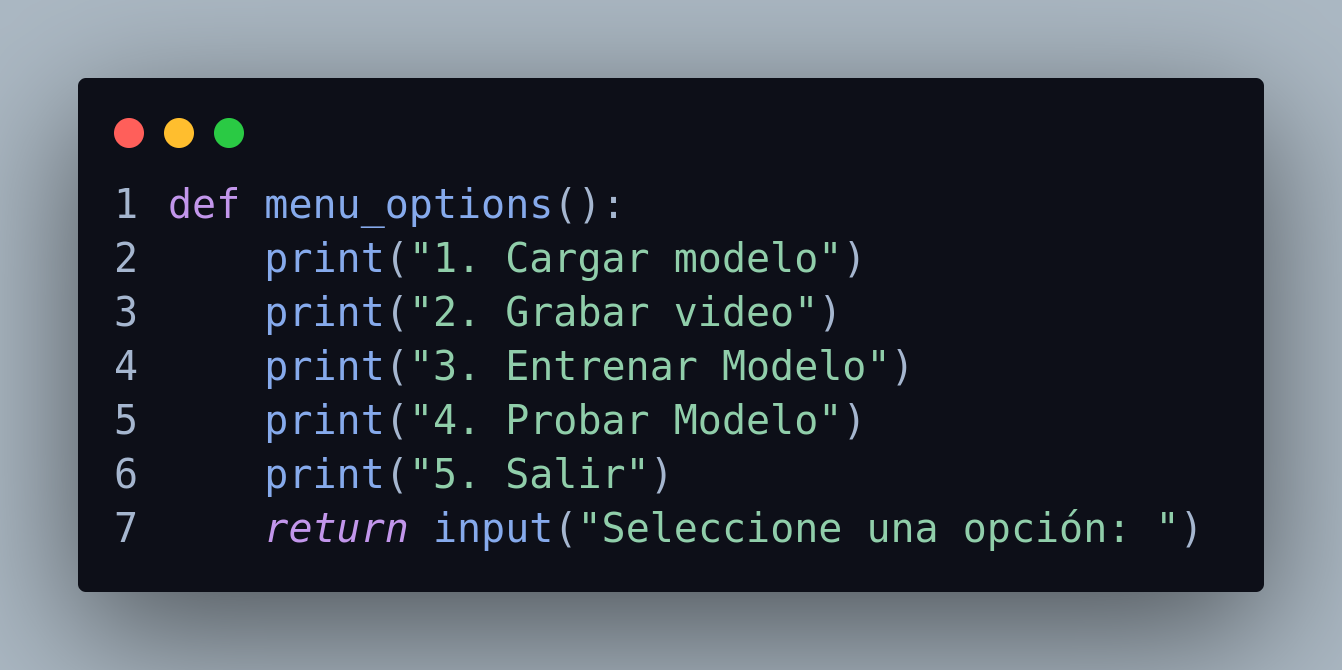
\includegraphics[width=0.8\linewidth]{imagenes/code.png}
    \caption{Menú por la terminal}
    \label{fig:enter-label}
\end{figure}

Esta manera de presentar las opciones hace que el uso del programa sea intuitivo ahorrandole al usuario tener conocimientos técnicos avanzados.

\subsection{Captura de imágenes}
Para entrenar este modelo es necesario recolectar y recopilar una base de datos para los rostros con sus respectivos códigos. Estos datos pueden ser recolectados mediante dos opciones:
\begin{itemize}
	{\bfseries\item Opción 1: Cargar modelo \par}
    {\normalsize El usuario tiene que proporcionar un archivo de video ya previamente grabado, indicando la ruta específica para este archivo. El sistema analiza el archivo de manera que recolecta cada fotograma (frame) del video para detectar los rostros presentes utilizando el algoritmo Haar Cascades. Ya con estos rostros identificados son almacenados en la carpeta faces como imágenes individuales acompañada del código de estudiante.}

    {\bfseries\item Opción 2: Grabar rostro\par}
    {\normalsize En esta opción, mediante el uso de la cámara integrada del dispositivo, los usuarios pueden capturar imágenes de sus rostros en tiempo real. Esta recolección se realiza al mantener presionada la tecla ‘p’, el sistema inicia guardando los rostros de los fotogramas entrantes. Cada rostro es guardado como una imagen con la etiqueta del código de estudiante. Esta opción se planea usar para registrar los rostros de manera inmediata y rápida sin necesidad de usar archivos externos.}
	
\end{itemize}


\subsection{Preprocesamiento de imágenes}
\begin{itemize}
	{\bfseries\item Conversión a escala de grises:} Las imágenes capturadas a color son convertidas a la escala de grises. Este cambio se traduce a la reducción de la cantidad de información innecesaria y mejora la velocidad del procesamiento sin afecta la calidad del reconocimiento.
	{\bfseries\item Redimensionamiento:} Todas las imágenes son ajustadas a un tamaño uniforme de 200 x 200 píxeles, esto garantiza la consistencia en la entrada al modelo mejorando la precisión y velocidad al no ser una resolución alta.
	{\bfseries\item Detección de rostros:} En este punto se aplica el algoritmo Harr Cascade para localizar las regiones de interés (rostros) en cada imagen. Estas zonas o regiones son las que se utilizan en el entrenamiento del modelo, aquí se descarta el fondo o los elementos irrelevantes \cite{khan2019face}.
\end{itemize}

\subsection{Entrenamiento del modelo}
Una vez que los datos ya fueron preparados en el preprocesamiento, se continúa con el entrenamiento del sistema de reconocimiento facial:
\begin{itemize}
	{\bfseries\item Modelo Eigenfaces:} El modelo EigenFaceRecognizer que es usado en este sistema, basado en el Análisis de Componentes Principales (PCA), reduce la dimensionalidad de las imágenes y extrae las características más representativas del rostro, conocidas como “eigenfaces”.
	{\bfseries\item Proceso de entrenamiento:} Las imágenes faciales y los códigos recolectados se usan en conjunto para el entrenamiento. El sistema aprende a distinguir los rostros y genera un archivo .xml que contiene los patrones faciales aprendidos. Este archivo se guarda como el modelo entrenado para su uso futuro \cite{ardila2022implementacion}.
\end{itemize}

\subsection{Prueba y reconocimiento}
Una vez el modelo se tiene entrenado, se pone a disposición el módulo \textit{4. Probar modelo}, para el reconocimiento facial en tiempo real
\begin{itemize}
	{\bfseries\item Detección en tiempo real:}Se activa la cámara del dispositivo y el sistema captura fotogramas continuos que son analizados para localizar rostros mediante Haar Cascade.
	{\bfseries\item Comparación con el modelo:}Cada modelo detectado se compara contra los patrones almacenados en archivo .xml. Se calcula un parámetro de confianza que indica que tan probable es que el rostro detectado corresponda a uno ya registrado.
	{\bfseries\item Visualización:} Este resultado se muestra en una ventana en tiempo real, donde cada rostro identificado anteriormente, aparece encerrado en un cuadrado de color azul, acompañado en la parte superior por el codigo y el nivel de confianza numerico.
\end{itemize}

\subsection{Ventajas del enfoque}
\begin{itemize}
    {\bfseries\item Eficiencia:} Gracias al previo procesamiento y el uso de los algoritmos optimizados como el PCA y Haar Cascades, el sistema ofrece un tiempo de respuesta aceptable inclusive en equipos con recursos limitados.
    {\bfseries\item Accesibilidad:} Al estar desarrollado completamente de Python y utilizar librerías de código abierto como OpenCv, el sistema es fácil de modificar, adaptar y expandir.
    {\bfseries\item Escalabilidad:} La estructura general del programa es modular y el uso de identificadores únicos permite que el sistemas escale y se expanda a nuevas personas, áreas académicas o incluso otras instituciones que requieran una solución para esta problemática.
\end{itemize}

%Desarrollo del programa
\section{Desarrollo del programama}
\subsection{main.py}
El archivo main sirve como núcleo central del programa, el cual proporciona una interfaz que muestra todas las funcionalidades.

El menú principal ofrece cinco opciones que cubren todo el flujo de trabajo del sistema de reconocimiento facial.
\begin{figure}[h]
    \centering
    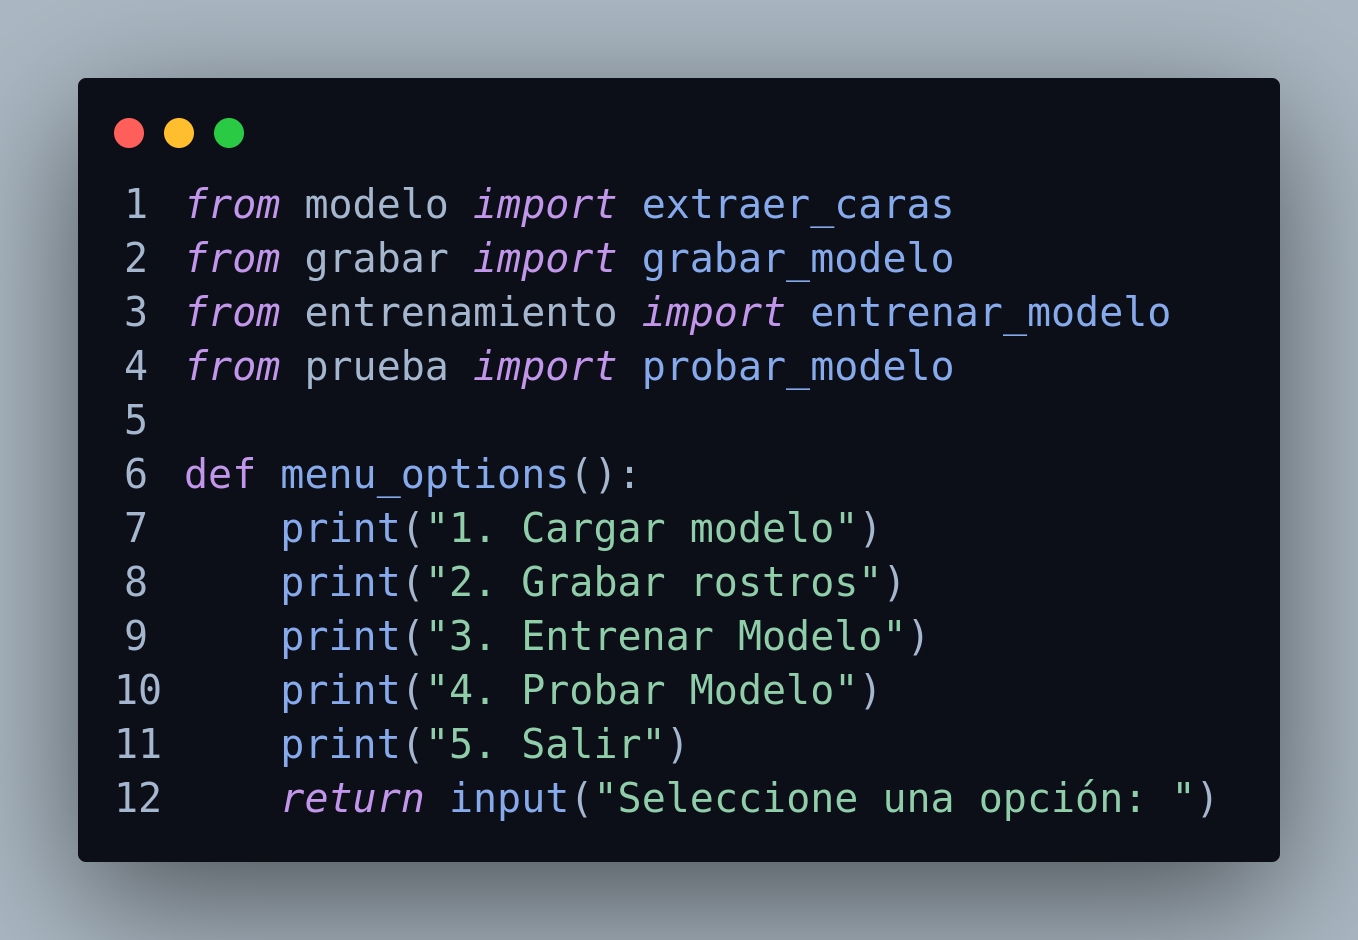
\includegraphics[width=0.8\linewidth]{imagenes/des01.png}
    \caption{Codigo menú principal}
    \label{fig:enter-label}
\end{figure}

El sistema de captura ofrece dos métodos (opción 1 y 2) para obtener imágenes faciales.

\subsection{Opcion 1: Cargar Modelo}

%Esta opcion se desarrolla en el archivo \textit{modelo.py}

%\begin{figure}
%    \centering
%    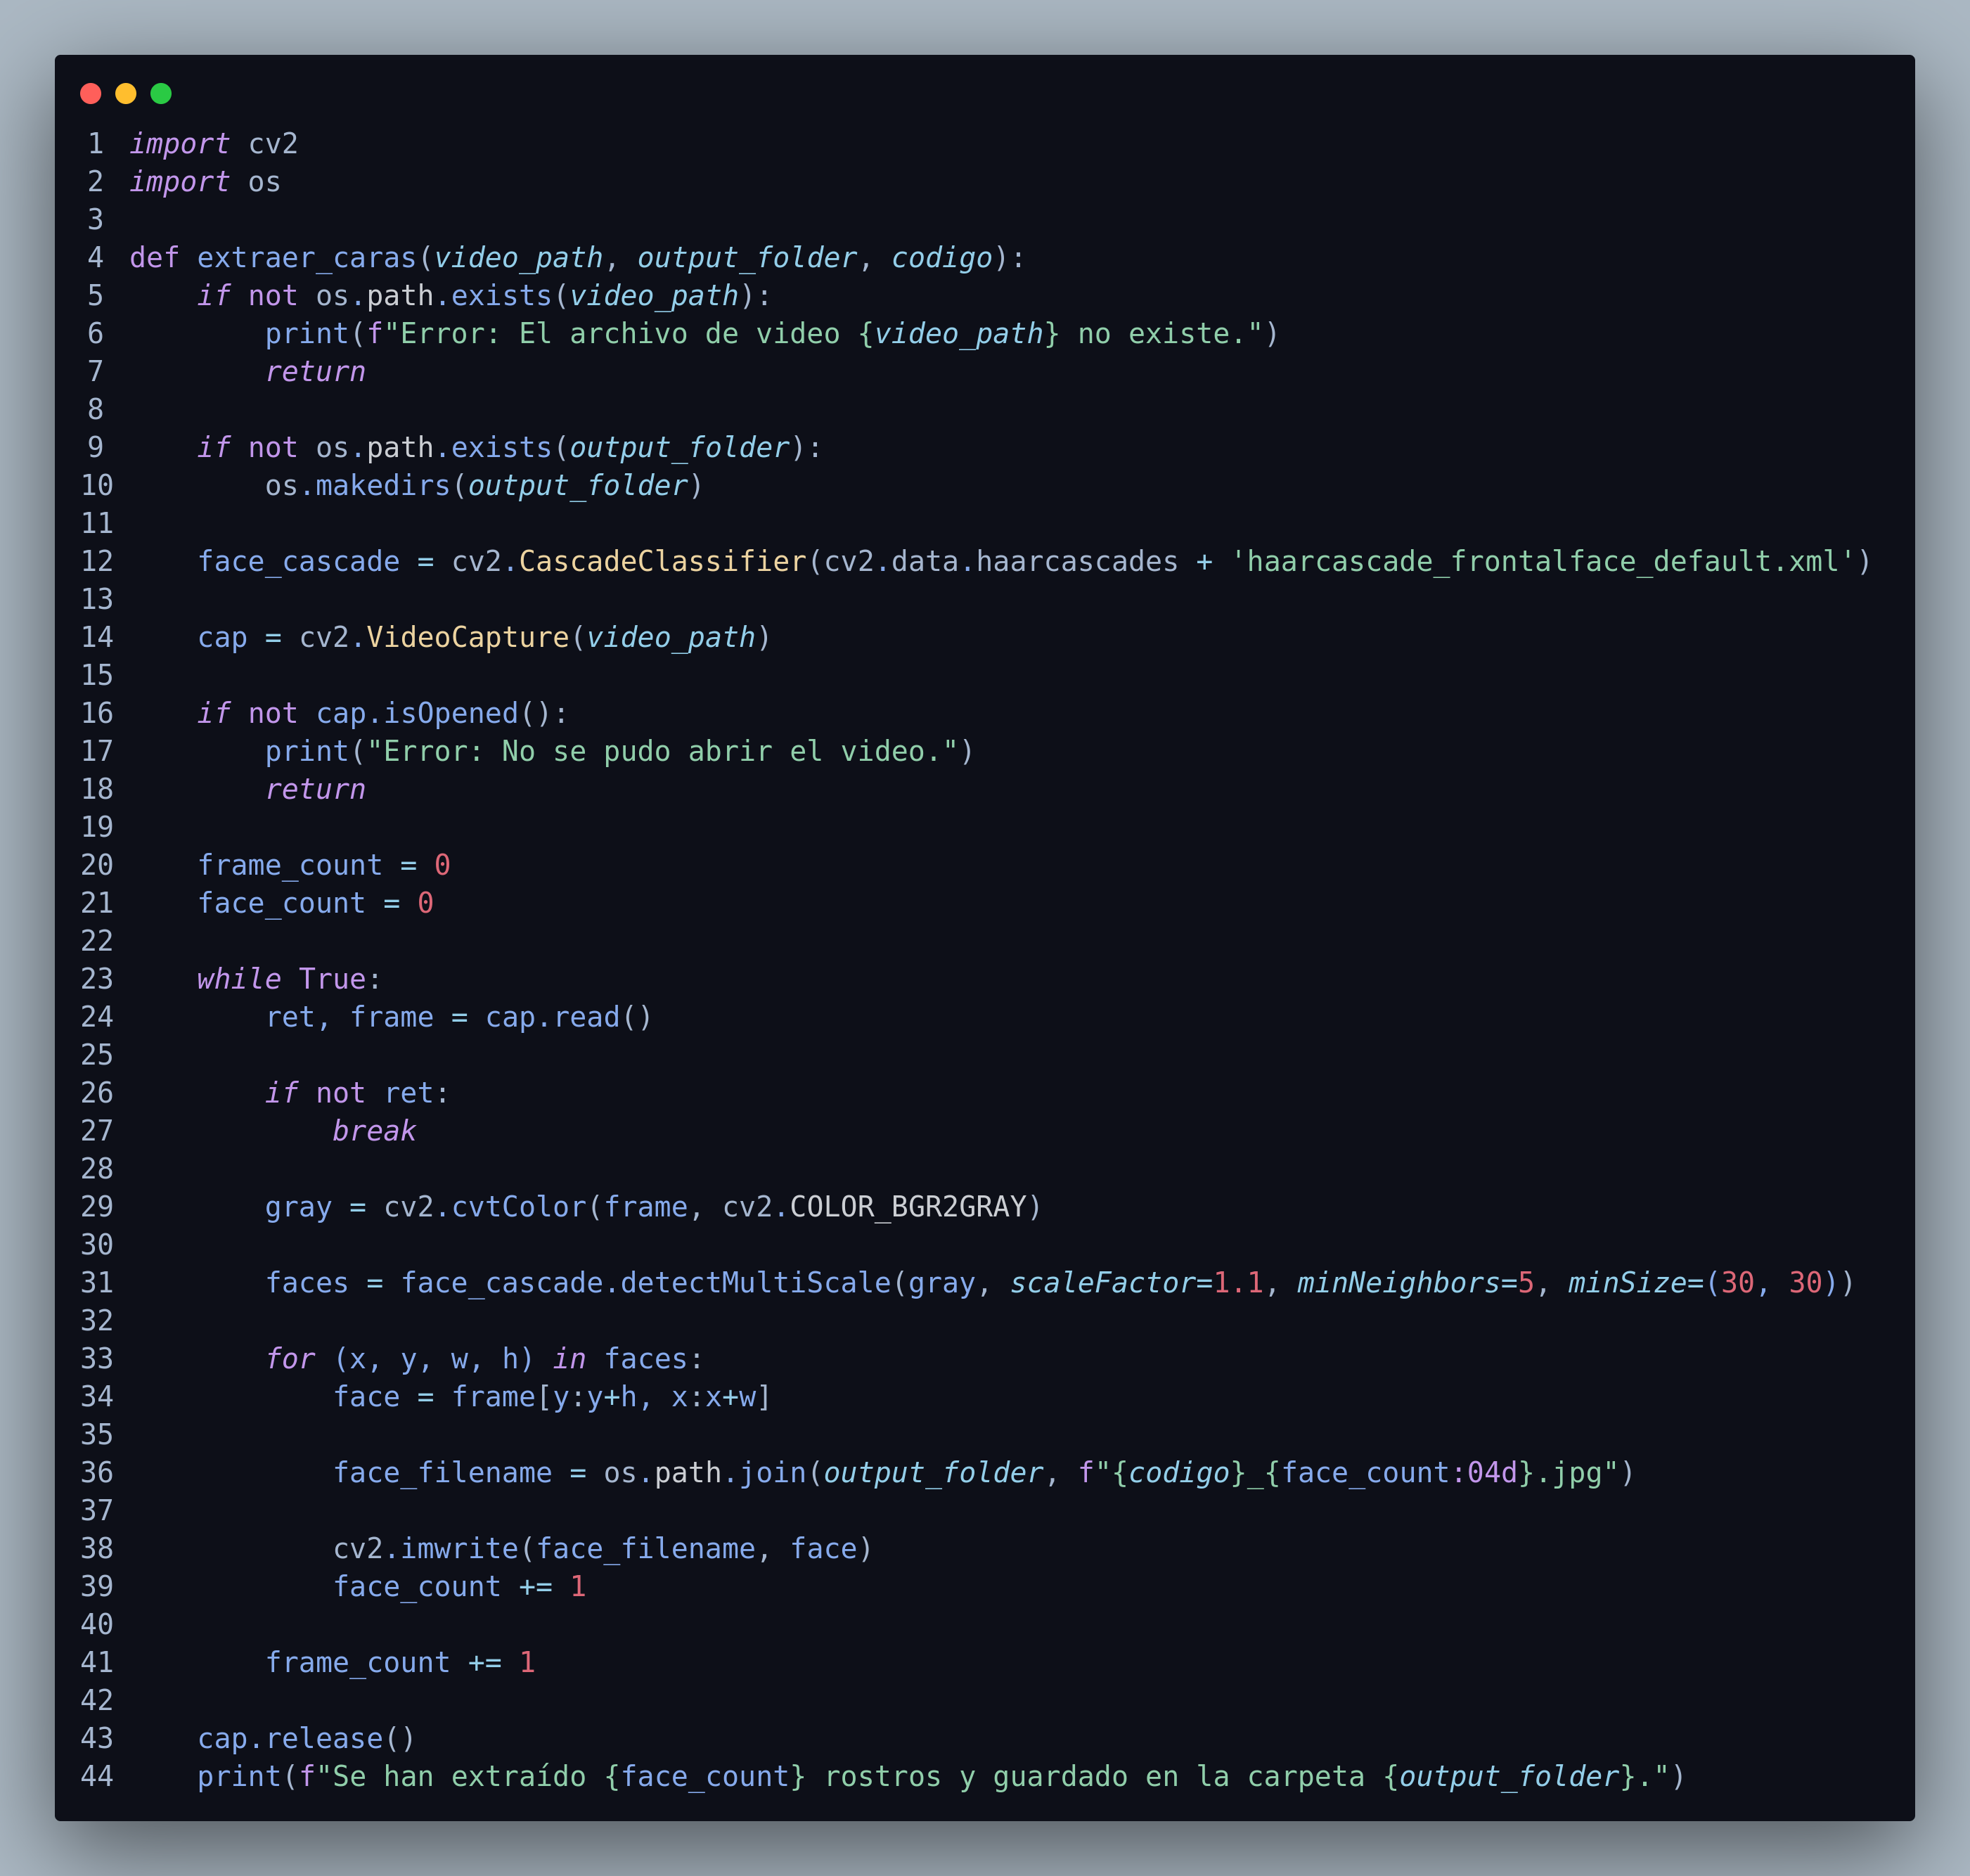
\includegraphics[width=1.0\linewidth]{imagenes/des00.png}
%    \caption{Codigo modelo.py}
%    \label{fig:enter-label}
%\end{figure}

Se importan las siguientes librerías CV2 y OS.

\begin{figure}[h]
    \centering
    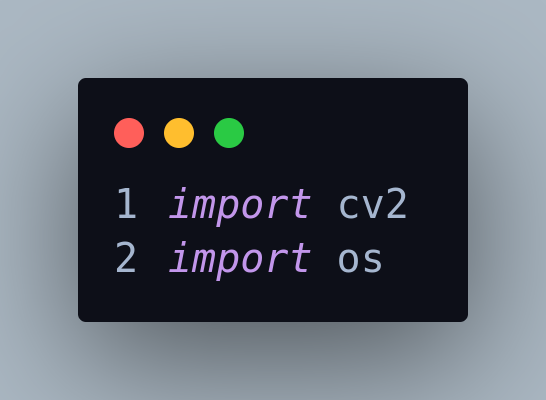
\includegraphics[width=0.4\linewidth]{imagenes/des02.png}
    \caption{Librerías CV2 y OS}
    \label{fig:enter-label}
\end{figure}

Se establece todo el código en una función para poder importarlo en el main, el cual tiene 3 parámetros los cuales reciben la ruta del video, el nombre de la carpeta donde se guardaran los rostros extraídos y el código del estudiante respectivamente.

\begin{figure}[h]
    \centering
    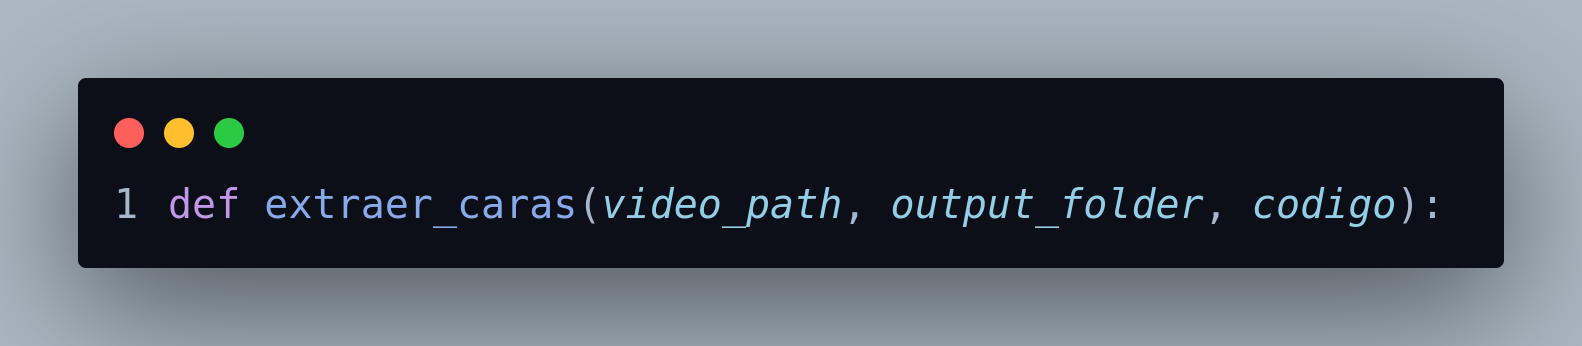
\includegraphics[width=0.75\linewidth]{imagenes/des03.png}
    \caption{Función extraer\_caras}
    \label{fig:enter-label}
\end{figure}

Utilizamos la función os.path.exists para comprobar si la ruta especificada apunta a un archivo existente en el sistema, la función termina inmediatamente si el archivo no existe; esta función también se usa para verificar si la carpeta de salida existe, y si no, la crea.

\begin{figure}[h]
    \centering
    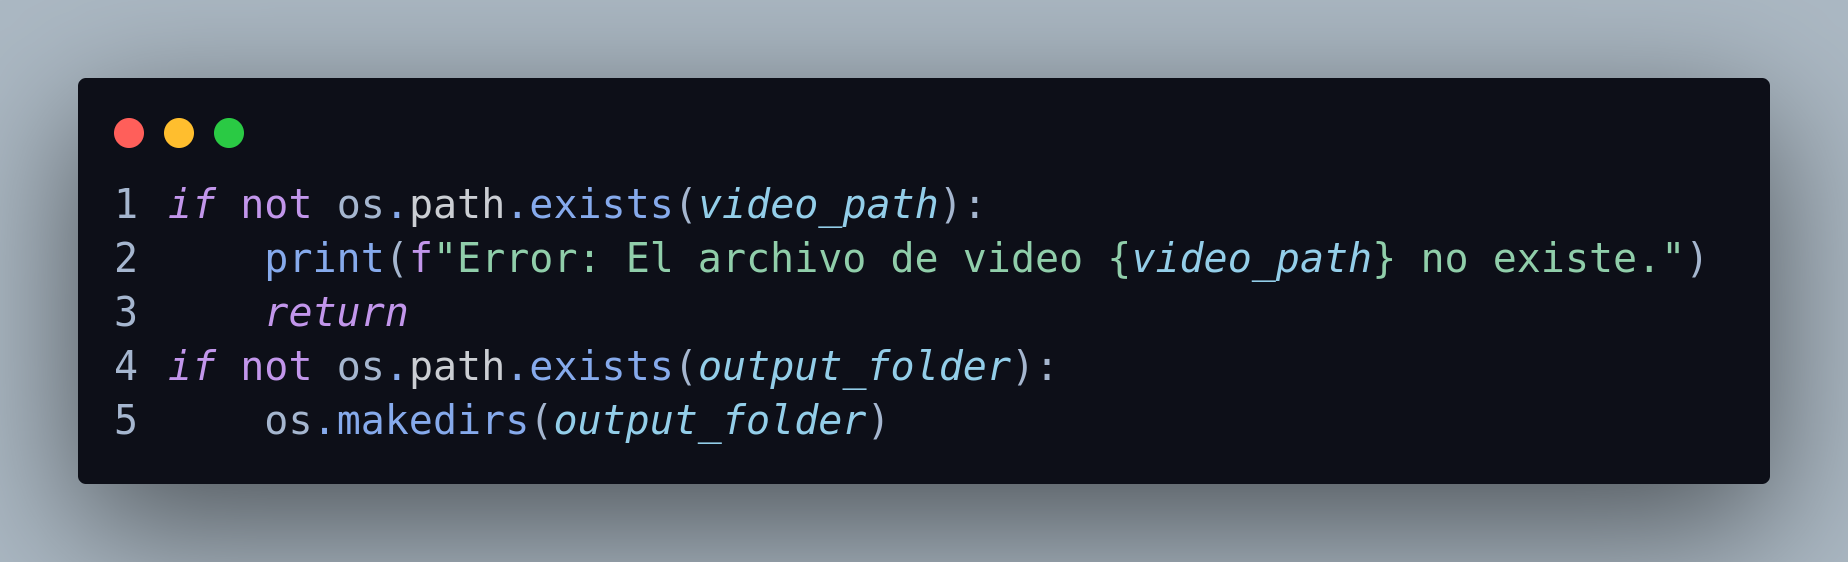
\includegraphics[width=0.9\linewidth]{imagenes/des04.png}
    \caption{Uso de os.path.exist}
    \label{fig:enter-label}
\end{figure}

Cargamos un clasificador preentrenado de Haar para la detección de rostros:

\begin{itemize}
    {\bfseries\item cv2.CascadeClassifier:} Carga clasificadores preentrenados basados en el algoritmo de cascada de Haar, estos clasificadores son modelos que pueden detectar objetos específicos (en este caso, rostros) en imágenes o videos.
    {\bfseries\item cv2.data.haarcascades:} Contiene la ruta al directorio donde se encuentran los clasificadores preentrenados de Haar.
    {\bfseries\item haarcascade\_frontalface\_default.xml:} Define las características que el clasificador utiliza para identificar rostros en una imagen.
\end{itemize}

\begin{figure}[h]
    \centering
    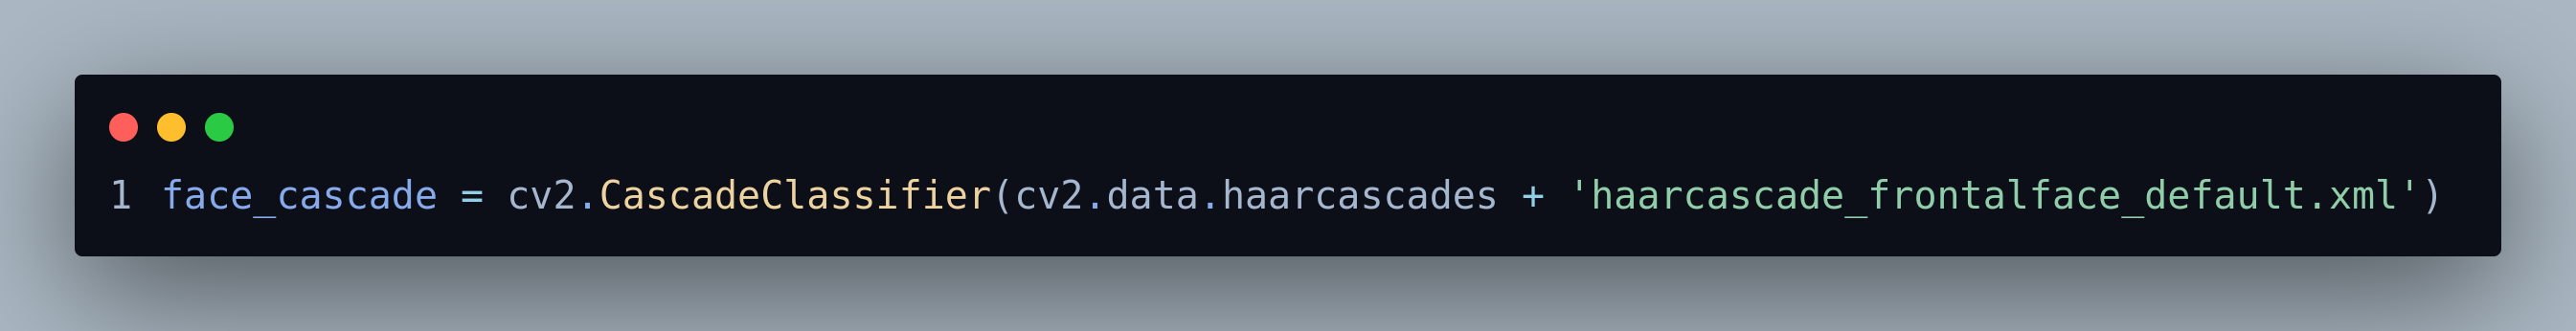
\includegraphics[width=1.0\linewidth]{imagenes/des05.png}
    \caption{Face\_cascade}
    \label{fig:enter-label}
\end{figure}

Usamos cv2.VideoCapture para capturar videos desde un archivo o una fuente de video en tiempo real, permite leer cuadros (frames) del video uno por uno para su procesamiento. Después de abrir el video, el código verifica si se pudo abrir correctamente.

\begin{figure}[h]
    \centering
    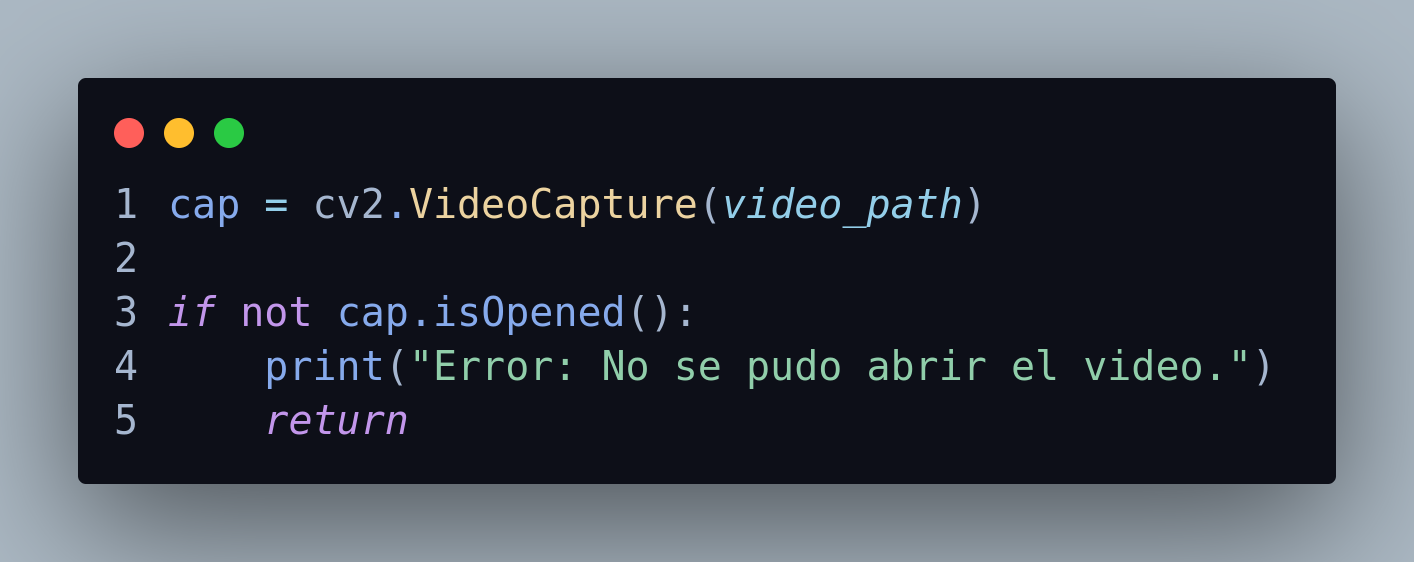
\includegraphics[width=0.80\linewidth]{imagenes/des06.png}
    \caption{cv2.VideoCapture}
    \label{fig:enter-label}
\end{figure}

Se establece un bucle para leer los cuadros del video, cap.read lee el siguiente cuadro del video, ret es un valor booleano que se detendrá cuando ya no halla mas cuadros en el video, frame contiene el cuadro actual del video como una imagen en formato de matriz (array) de OpenCV.

\begin{figure}[h]
    \centering
    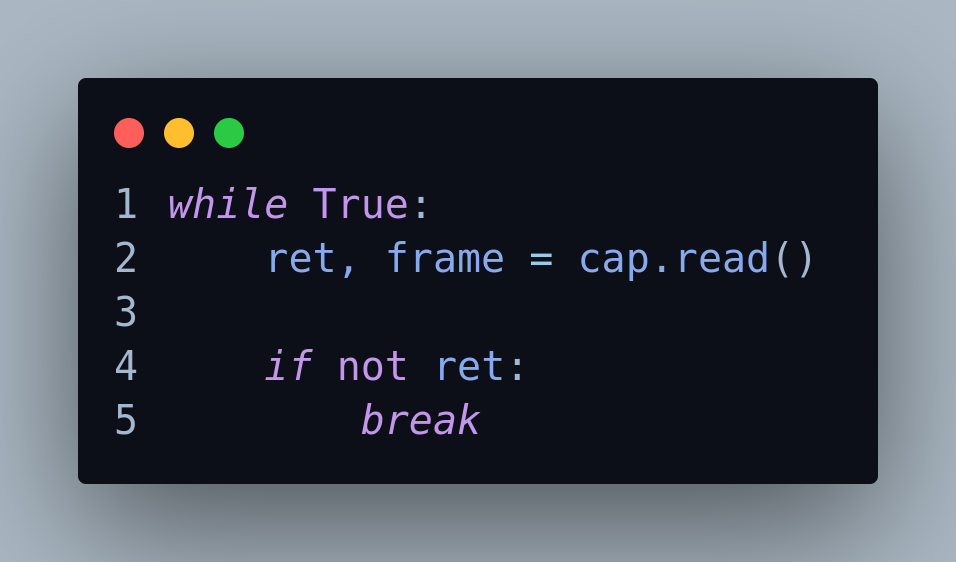
\includegraphics[width=0.66 \linewidth]{imagenes/des07.png}
    \caption{Bucle para cap.read}
    \label{fig:enter-label}
\end{figure}

La función cv2.cvtColor convierte el cuadro actual de BGR a escala de grises, la detección de rostros con Haar Cascades funciona mejor en imágenes en esa escala, ya que reduce la complejidad computacional y elimina la información de color innecesaria. 

\begin{itemize}
    {\bfseries\item face\_cascade.detectMultiScale:} Detecta rostros en la imagen en escala de grises.
    {\bfseries\item scaleFactor = 1.1:} Especifica cuánto se reduce el tamaño de la imagen en cada escala, un 10\% en cada iteración.
    {\bfseries\item minNeighbors = 5:} Mínimo de vecinos que deben ser detectados para que una región sea considerada un rostro. Un valor más alto reduce las detecciones falsas.
    {\bfseries\item minSize  = (30, 30):} Tamaño mínimo de los rostros que se detectarán.
\end{itemize}

\begin{figure}[h]
    \centering
    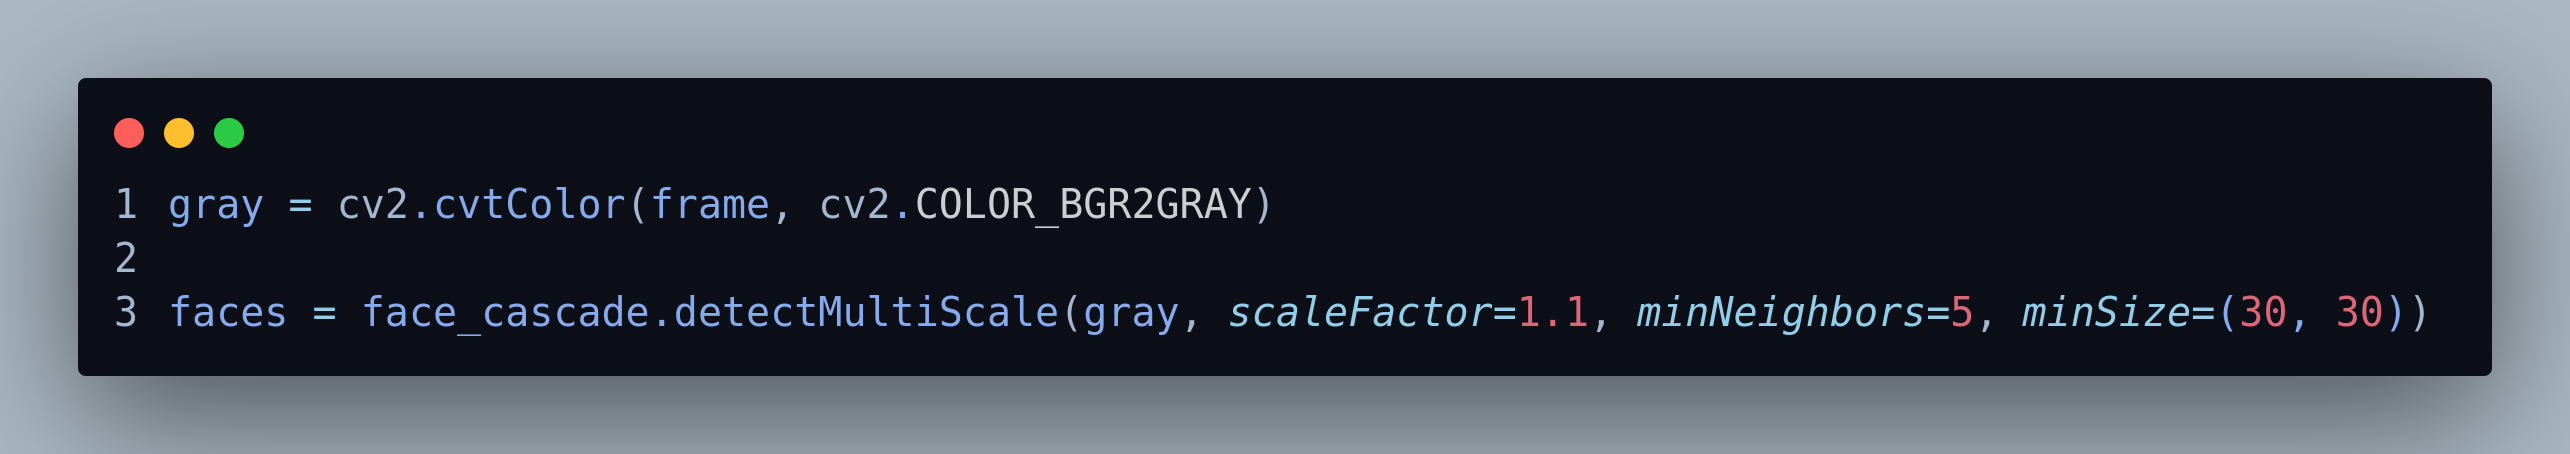
\includegraphics[width=1.0\linewidth]{imagenes/des08.png}
    \caption{ingresar caption}
    \label{fig:enter-label}
\end{figure}

El resultado de esta función es una lista de coordenadas de los rostros detectados en el cuadro actual. Cada rostro se representa como un rectángulo con las coordenadas (x, y, w, h).

Procesamos cada rostro detectado en un cuadro del video, lo recorta, (x, y) (esquina superior izquierda) y el tamaño (w, h) (ancho y alto del rectángulo),con cv2.imwrite(face\_filename, face) se guarda como una imagen en la carpeta de salida y actualiza los contadores.

\begin{itemize}
    {\bfseries\item f"{codigo}\_{face\_count:04d}.jpg":} Asegura que el número del rostro con 4 dígitos, rellenando con ceros a la izquierda si es necesario.
\end{itemize}

\begin{figure}[h]
    \centering
    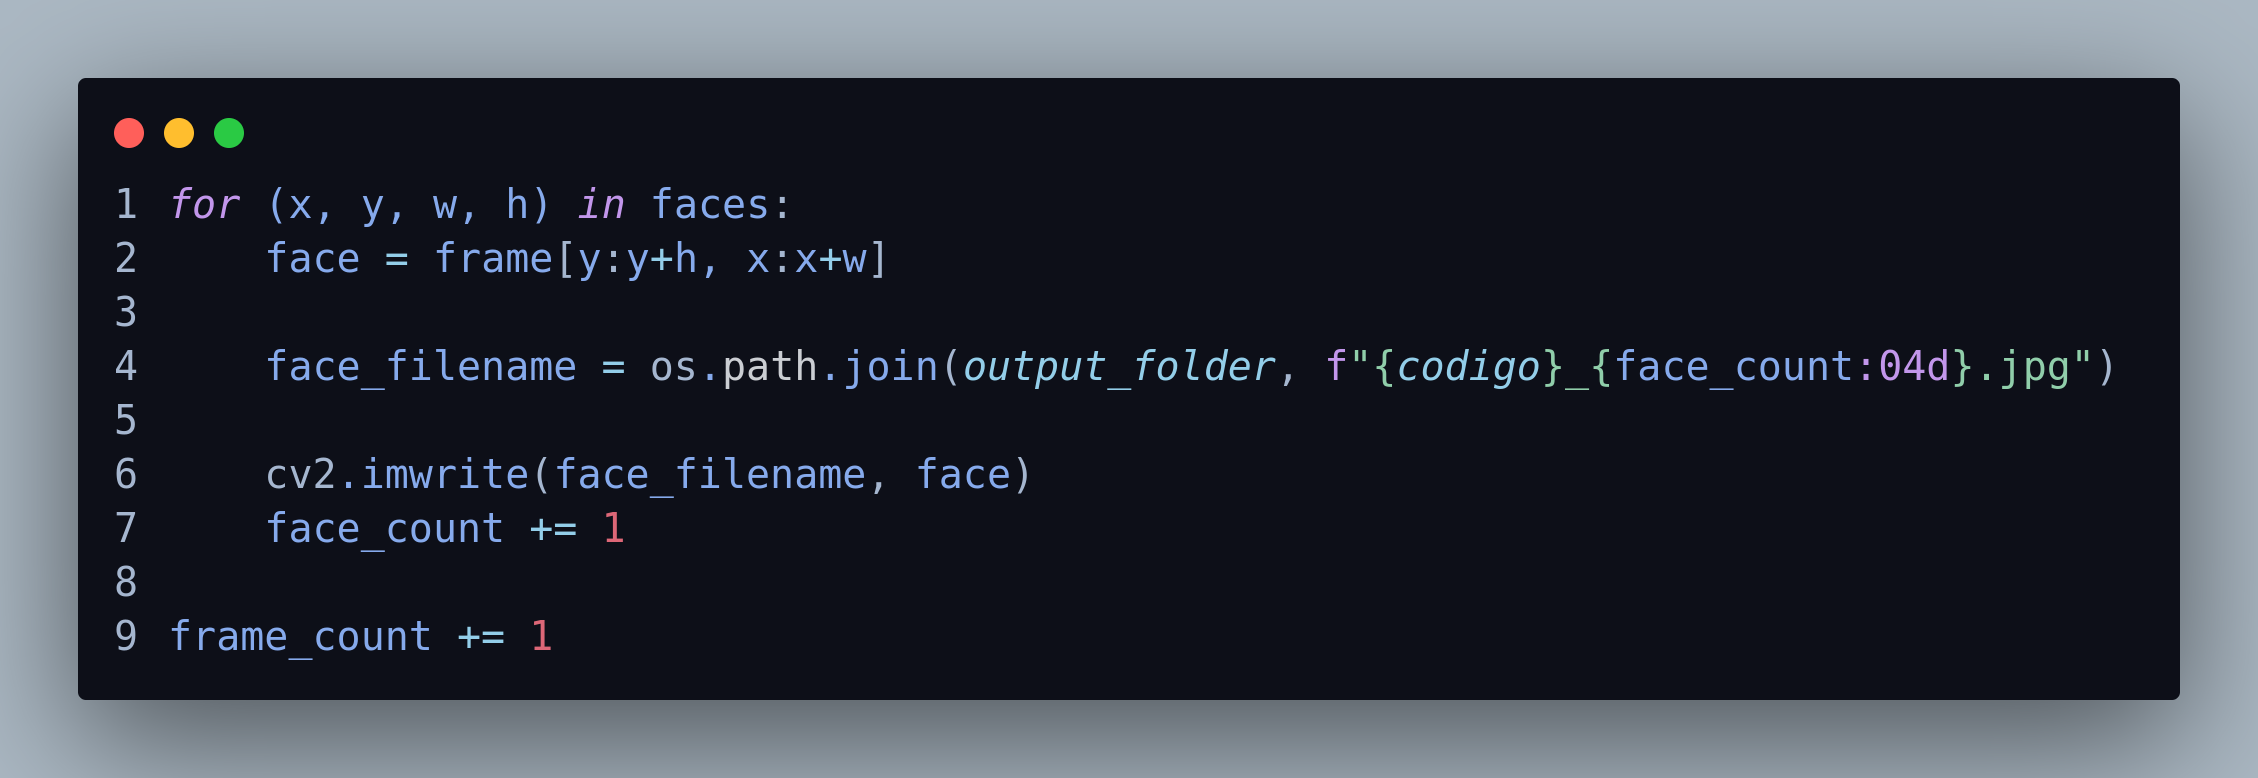
\includegraphics[width=1.0\linewidth]{imagenes/des09.png}
    \caption{ingresar caption}
    \label{fig:enter-label}
\end{figure}

Al final cap.release se asegura que el video se cierre correctamente y que los recursos del sistema no queden bloqueados.

\begin{figure}[h]
    \centering
    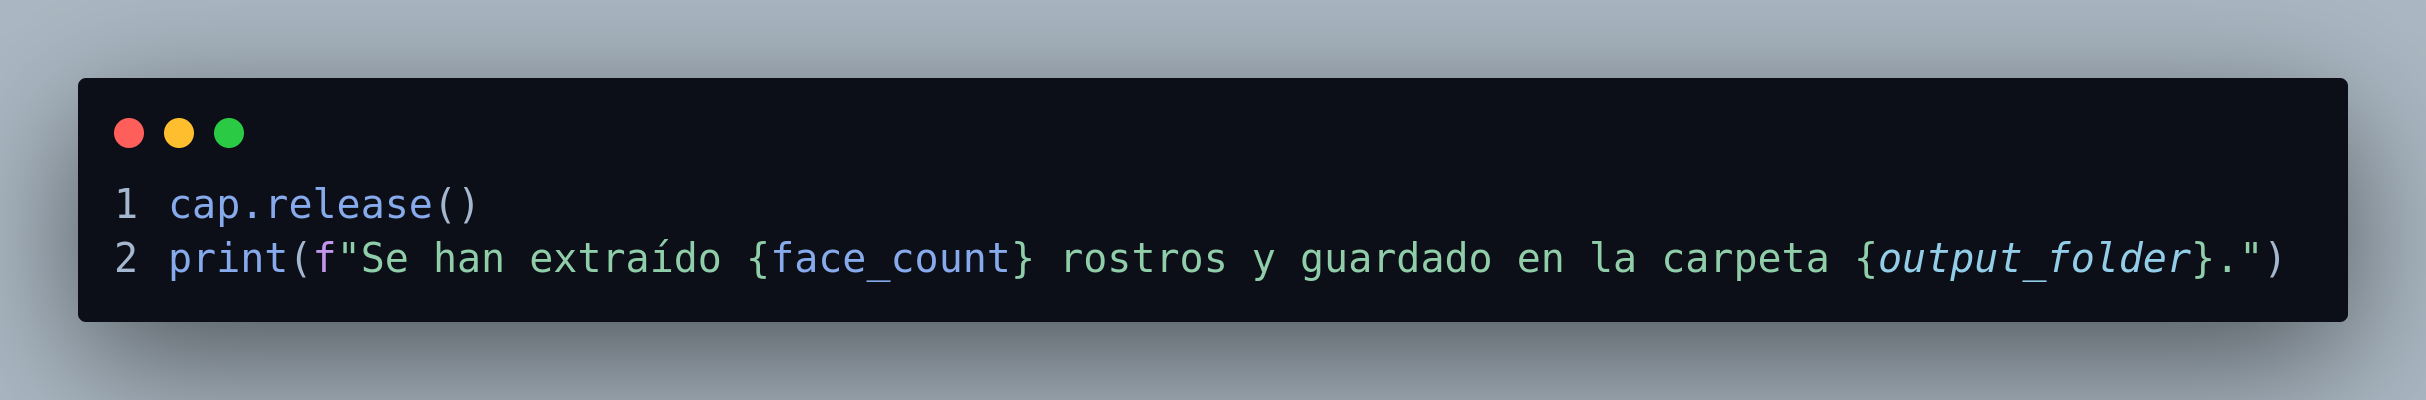
\includegraphics[width=1.0\linewidth]{imagenes/des10.png}
    \caption{ingresar caption}
    \label{fig:enter-label}
\end{figure}

\subsection{Opcion 2: Grabar Rostros}
Esta opción ofrece una alternativa de captura en tiempo real mediante la cámara web. Aunque comparte algunos elementos técnicos con la primera opción, como el uso de un bucle para leer los frames y el uso del clasificador Haar Cascade, su implementación presenta diferencias clave en el flujo de trabajo y la interacción con el usuario.

A diferencia de la Opción 1 que usa un archivo de video, aquí se accede directamente al flujo de video en vivo.

\begin{itemize}
    {\bfseries\item 0:} Es el índice de la cámara que se desea usar. En la mayoría de los sistemas, 0 se refiere a la cámara predeterminada, si se tiene múltiples cámaras conectadas, se puede usar 1, 2, etc., para seleccionar otras cámaras.
\end{itemize}

\begin{figure}[h]
    \centering
    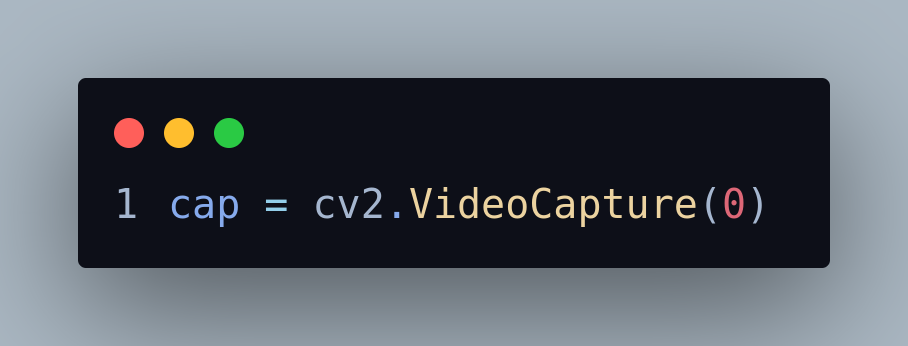
\includegraphics[width=0.5\linewidth]{imagenes/des11.png}
    \caption{ingresar caption}
    \label{fig:enter-label}
\end{figure}

Se muestra el video en tiempo real y se transforma el frame en escala de grises.

\begin{figure}[h]
    \centering
    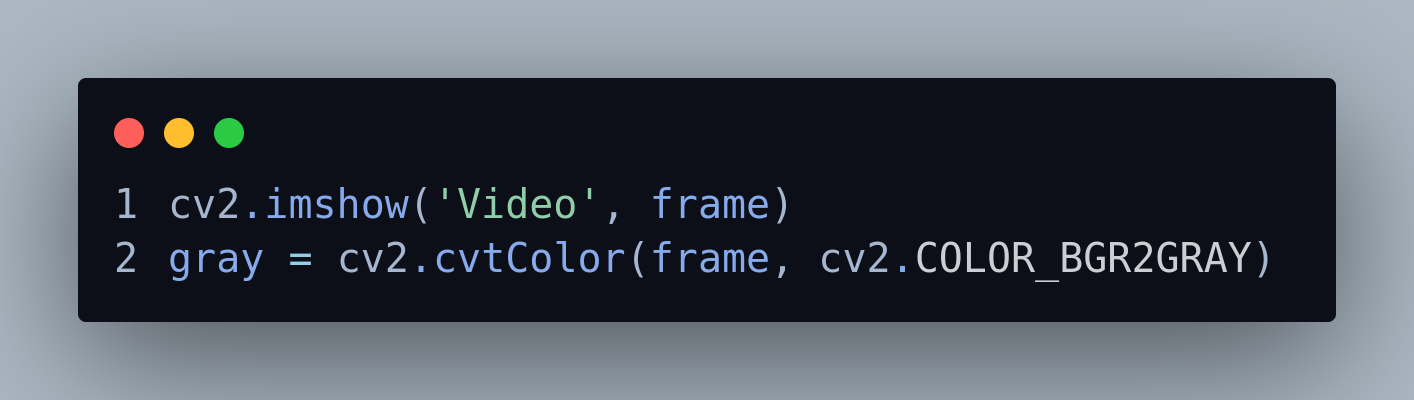
\includegraphics[width=0.75\linewidth]{imagenes/des12.png}
    \caption{ingresar caption}
    \label{fig:enter-label}
\end{figure}

La tecla 'p' activa la captura de rostros cuando se mantiene presionada 

\begin{itemize}
    {\bfseries\item cv2.waitKey(1):} Espera 1 milisegundo para detectar si se ha presionado una tecla.
    {\bfseries\item ord("p"):} Convierte el carácter \texttt{"p"} en su valor ASCII.
\end{itemize}

\begin{figure}[h]
    \centering
    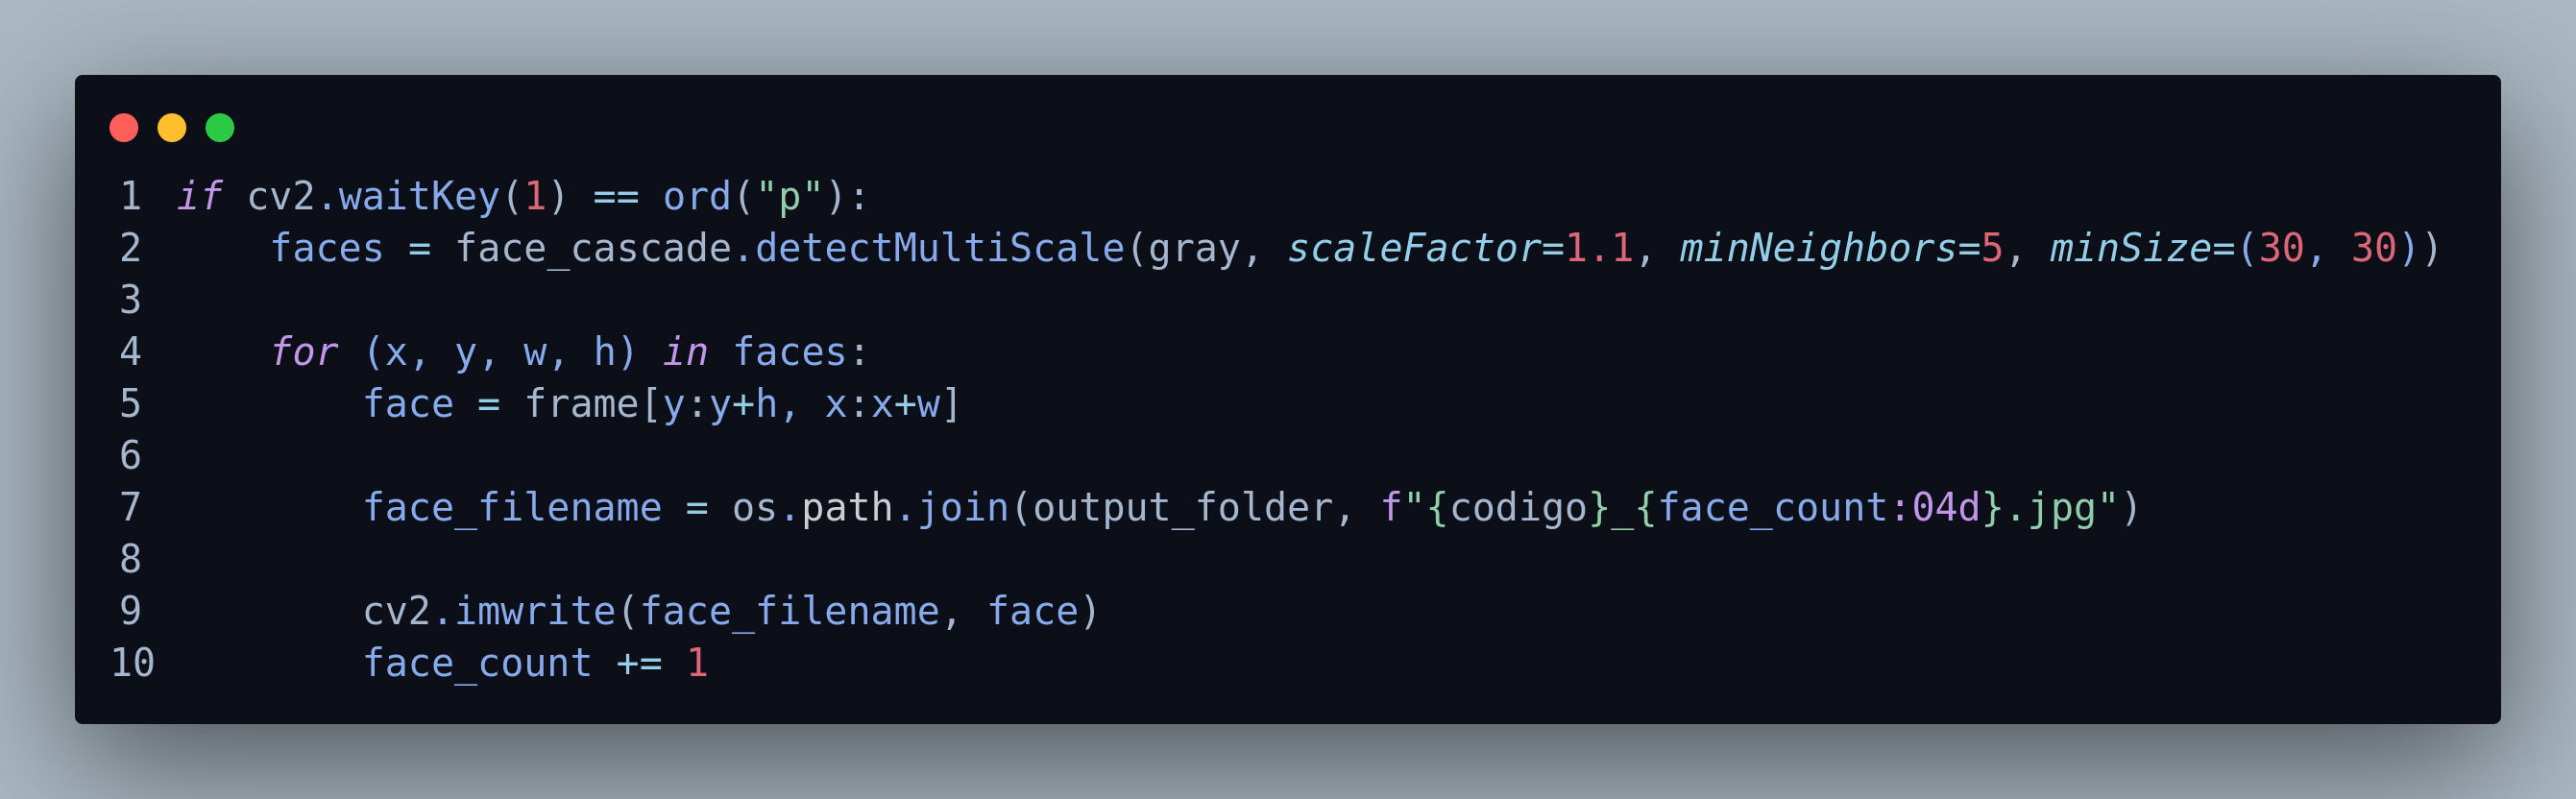
\includegraphics[width=1.0\linewidth]{imagenes/des13.png}
    \caption{ingresar caption}
    \label{fig:enter-label}
\end{figure}

La tecla 'q' finaliza el proceso deteniendo la captura de video.

\begin{figure}[h]
    \centering
    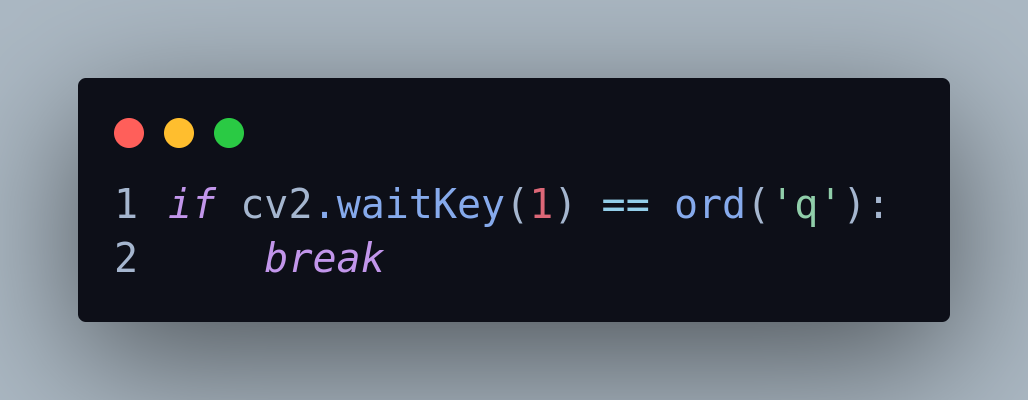
\includegraphics[width=0.65\linewidth]{imagenes/des14.png}
    \caption{ingresar caption}
    \label{fig:enter-label}
\end{figure}

\begin{itemize}
    {\bfseries\item cv2.destroyAllWindows(): } Cierra todas las ventanas abiertas por OpenCV, como la ventana que muestra el video en tiempo real, esto limpia la interfaz gráfica y evita que queden ventanas abiertas después de que el programa termine.
\end{itemize}

\begin{figure}[h]
    \centering
    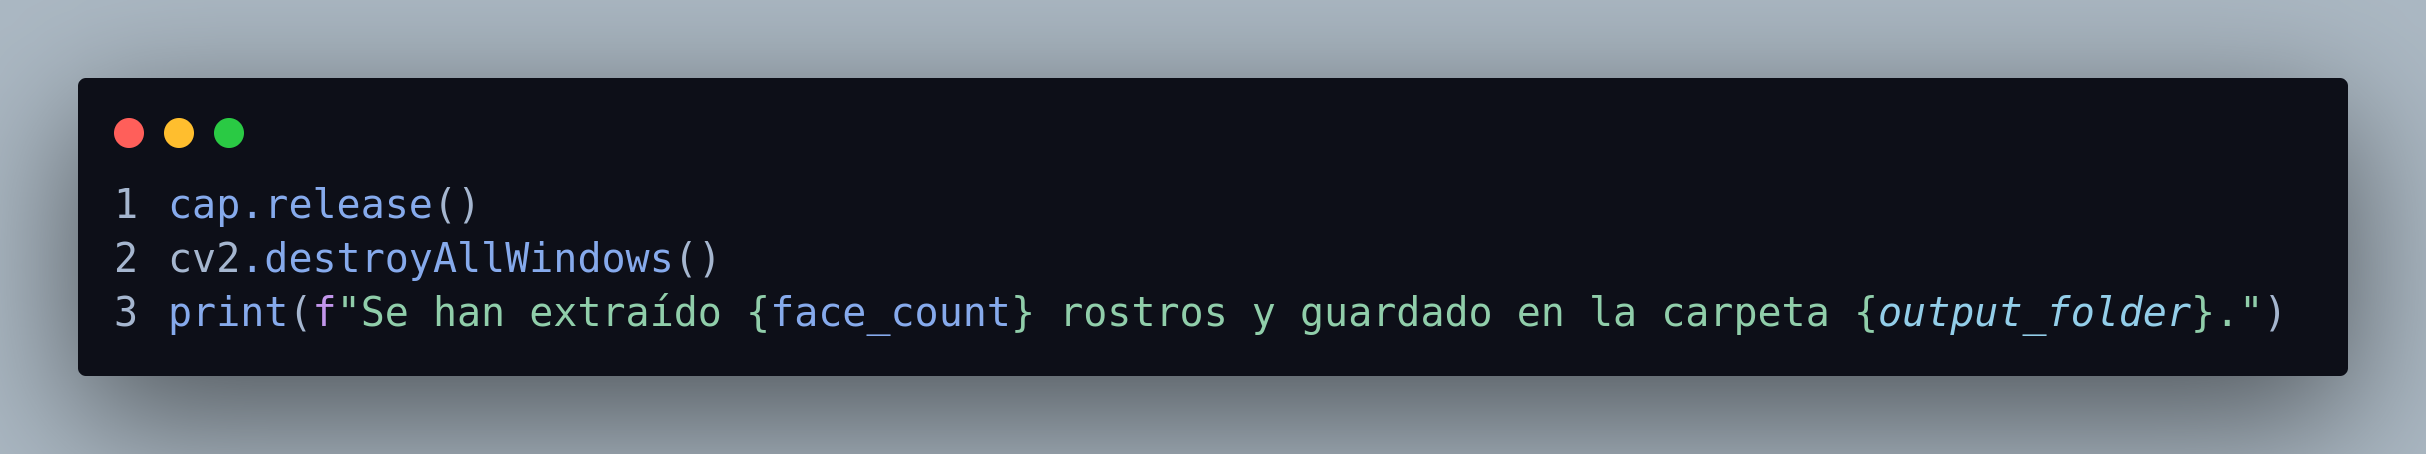
\includegraphics[width=1.0\linewidth]{imagenes/des15.png}
    \caption{Caption}
    \label{fig:enter-label}
\end{figure}

\subsection{Opcion 3: Entrenar Modelo}

Se importan las siguientes librerías

\begin{figure}[h]
    \centering
    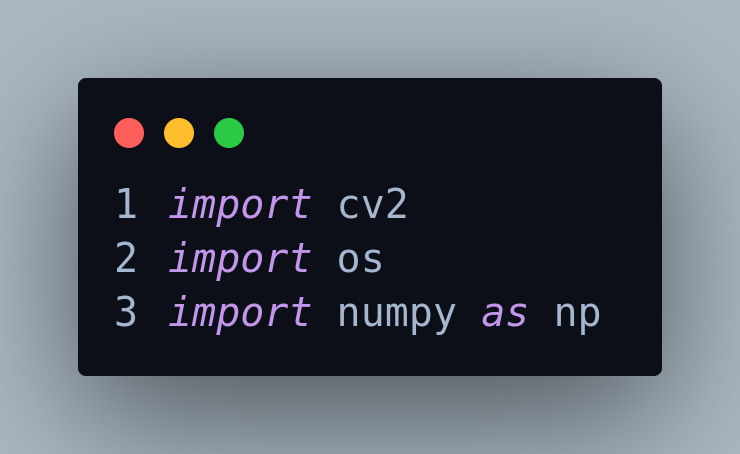
\includegraphics[width=0.5\linewidth]{imagenes/des17.png}
    \caption{ingresar caption}
    \label{fig:enter-label}
\end{figure}

Se define la carpeta donde están almacenadas las imágenes de entrenamiento. En este caso, la carpeta se llama 'faces'. Se llama a la función cargar imágenes. 

\begin{figure}[h]
    \centering
    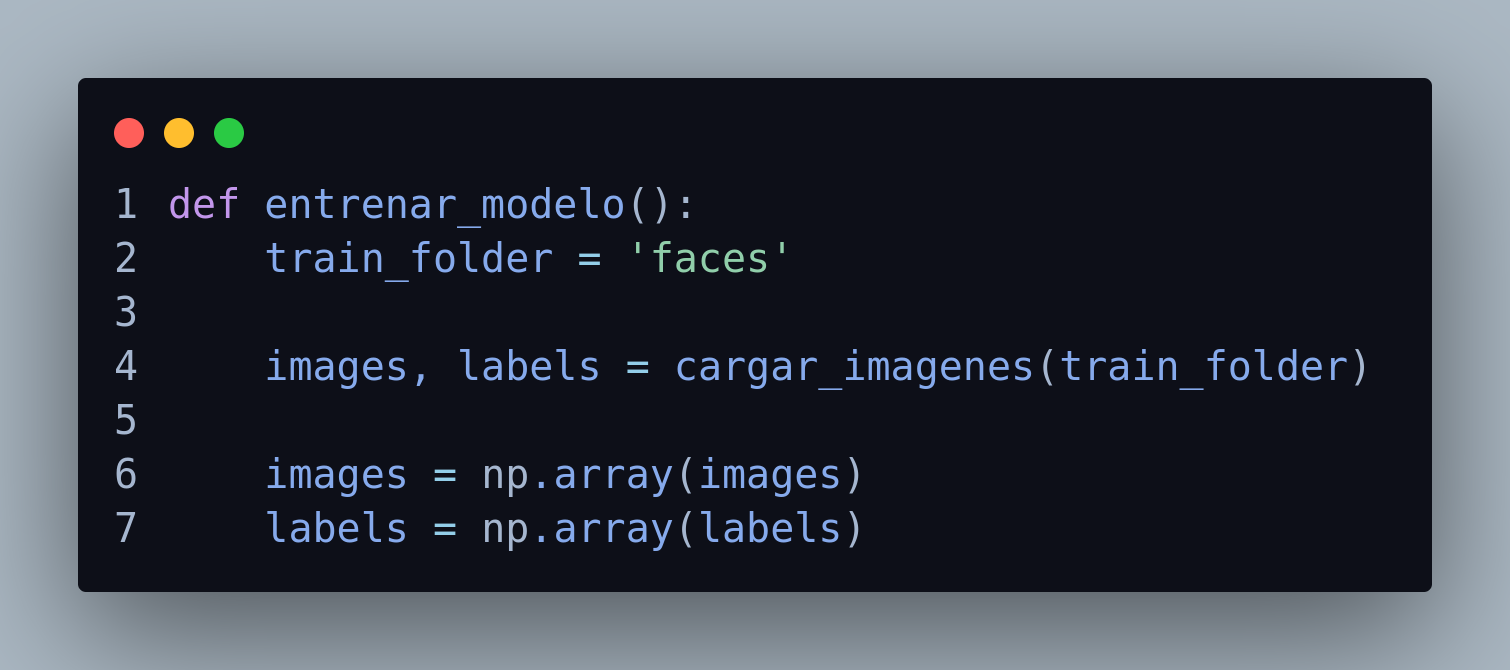
\includegraphics[width=0.9\linewidth]{imagenes/des18.png}
    \caption{Caption}
    \label{fig:enter-label}
\end{figure}

Esta funcion recibe la ruta de la carpeta donde se encuentran las imágenes e \textit{image\_size = (200,200)} que es el tamaño al que se redimensionarán las imágenes, por defecto, \textit{200x200 píxeles}. Crea dos etiquetas vacías para guardar las imágenes y los códigos se itera sobre todos los archivos en la carpeta especificada.

\begin{itemize}
    {\bfseries\item os.path.join(folder, filename):} Construye la ruta completa del archivo combinando la carpeta y el nombre del archivo.
    {\bfseries\item cv2.imread(img\_path, cv2.IMREAD\_GRAYSCALE):} Para leer la imagen en escala de grises.
    {\bfseries\item os.path.basename(filename).split('\_')[0]:} Extrae la etiqueta de la imagen a partir del nombre del archivo.
\end{itemize}

\begin{figure}[h]
    \centering
    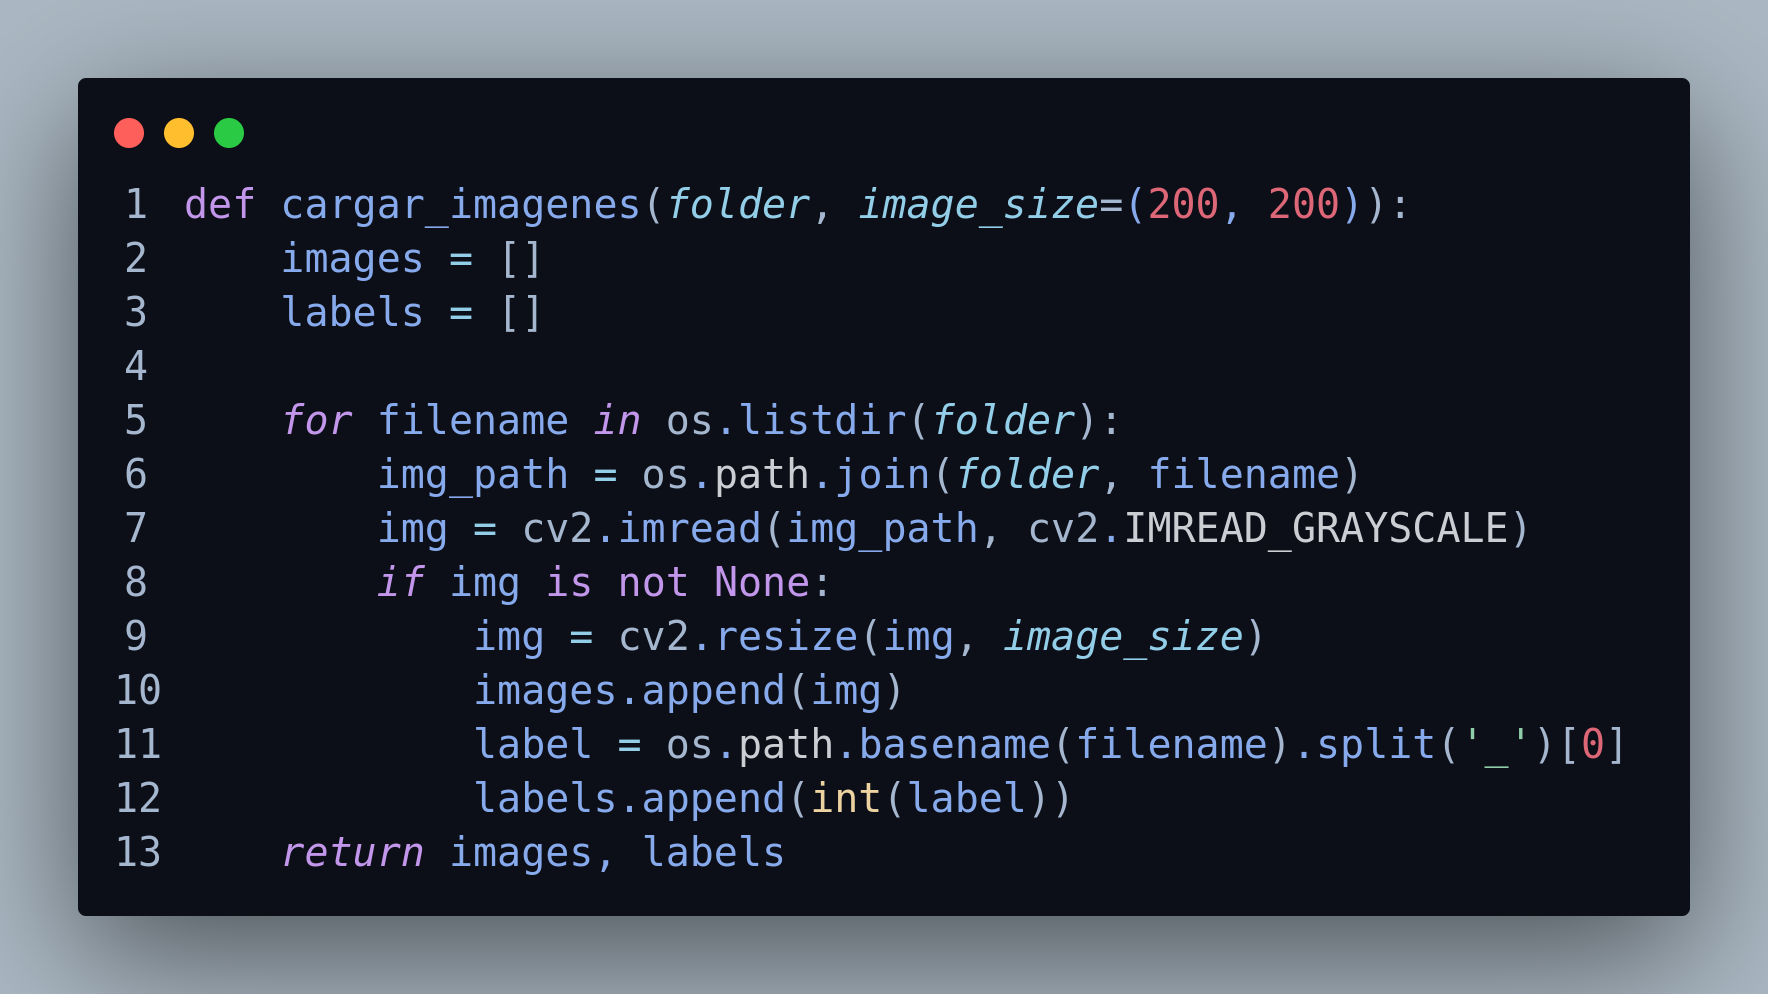
\includegraphics[width=0.85\linewidth]{imagenes/des19.png}
    \caption{Ingresar caption}
    \label{fig:enter-label}
\end{figure}

Se crea un modelo de reconocimiento facial utilizando la clase EigenFaceRecognizer, se entrena el modelo y se guarda como 'eigenfaces\_model.xml'

\begin{itemize}
    {\bfseries\item cv2.face:} Es un módulo de OpenCV que contiene herramientas específicas para el reconocimiento facial. Este módulo incluye varios algoritmos de reconocimiento facial, como Eigenfaces, Fisherfaces y Local Binary Patterns Histograms (LBPH). 
    {\bfseries\item EigenFaceRecognizer\_create:} Es un método que crea un modelo basado en el algoritmo de Eigenfaces. Este algoritmo utiliza Análisis de Componentes Principales (PCA) para reducir la dimensionalidad de las imágenes faciales y encontrar las características más relevantes para distinguir entre diferentes rostros.
\end{itemize}

\begin{figure}[h]
    \centering
    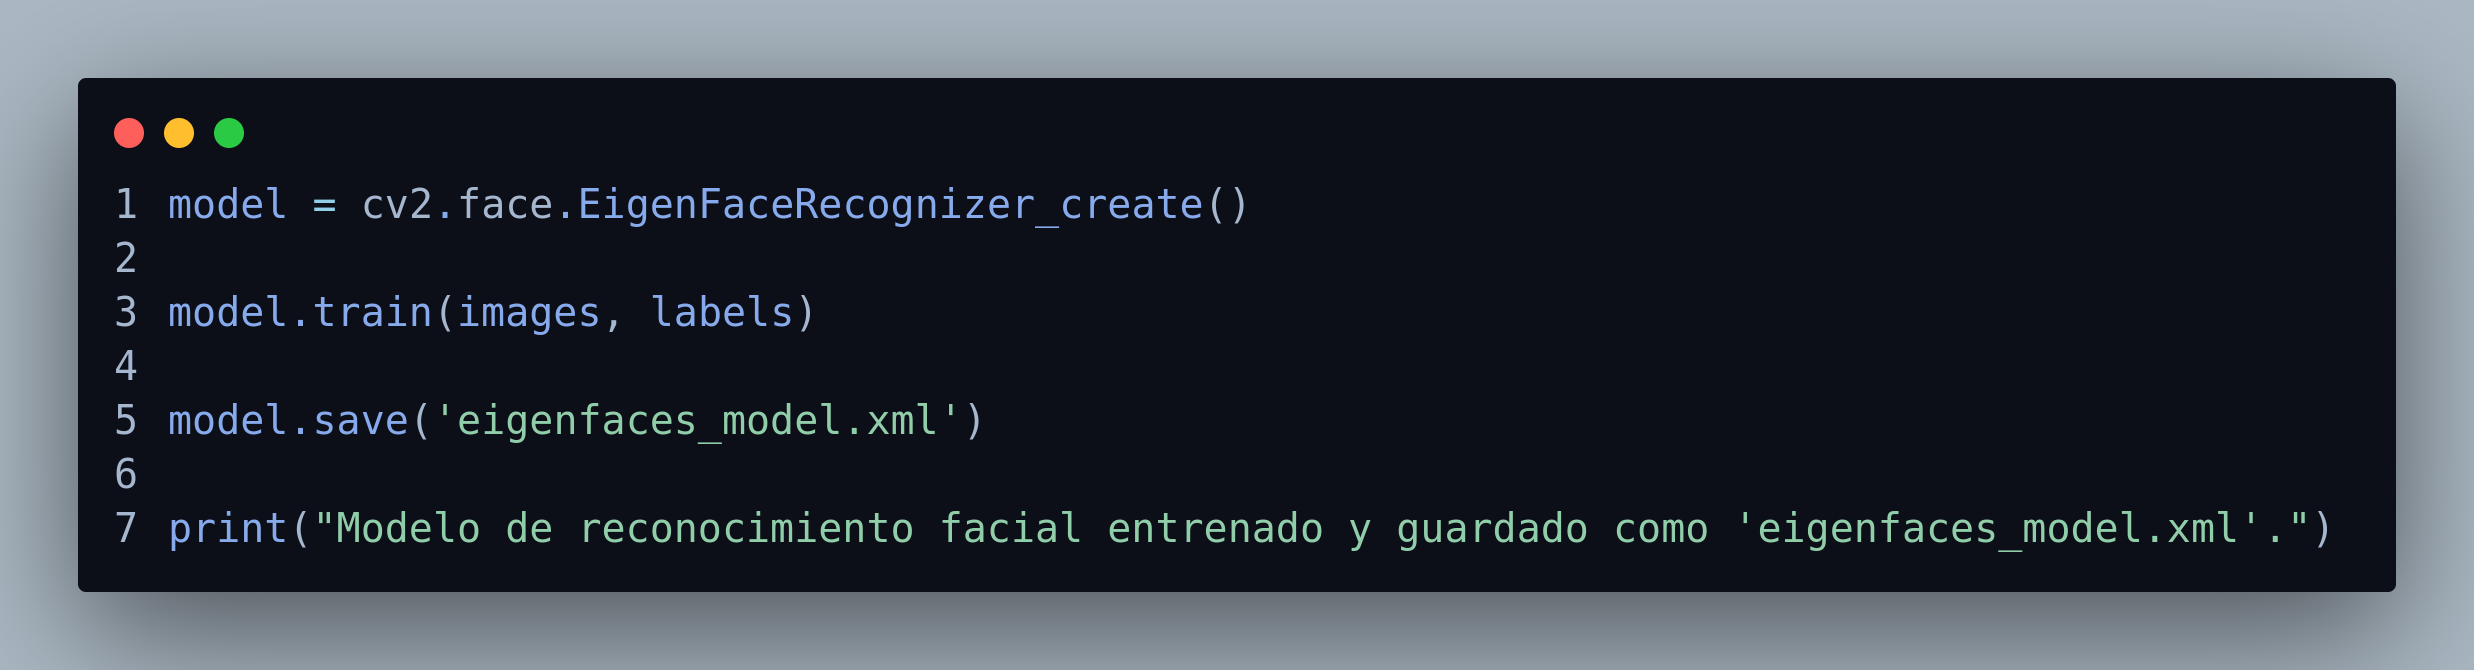
\includegraphics[width=1.0\linewidth]{imagenes/des20.png}
    \caption{Ingresar caption}
    \label{fig:enter-label}
\end{figure}

\subsection{Opcion 4: Probar Modelo}
La función comienza creando y cargando un modelo de reconocimiento facial basado en EigenFaces.

\begin{itemize}
    {\bfseries\item model.read('eigenfaces\_model.xml'):} Aquí se carga un modelo preentrenado, este archivo contiene los datos necesarios para que el modelo pueda realizar predicciones, como los vectores de características y los identificadores asociados a las imágenes de entrenamiento.
\end{itemize}

\begin{figure}[h]
    \centering
    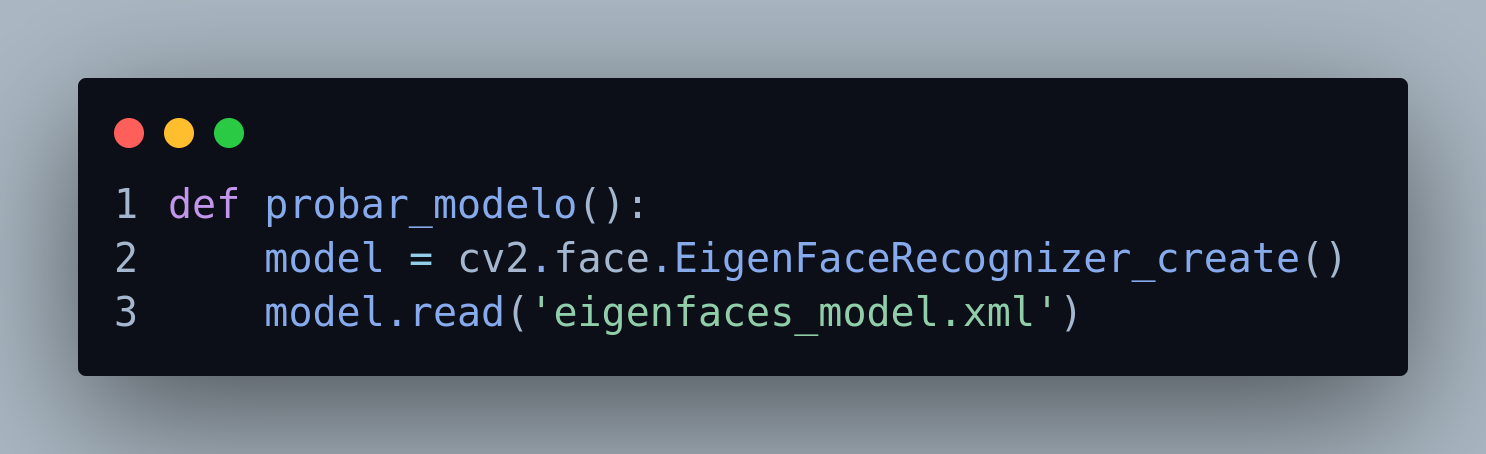
\includegraphics[width=0.65\linewidth]{imagenes/des22.png}
    \caption{Ingresar caption}
    \label{fig:enter-label}
\end{figure}

Se inicia la captura de video desde la cámara predeterminada y cargamos un clasificador en cascada preentrenado para la detección de rostros.

\begin{figure}[h]
    \centering
    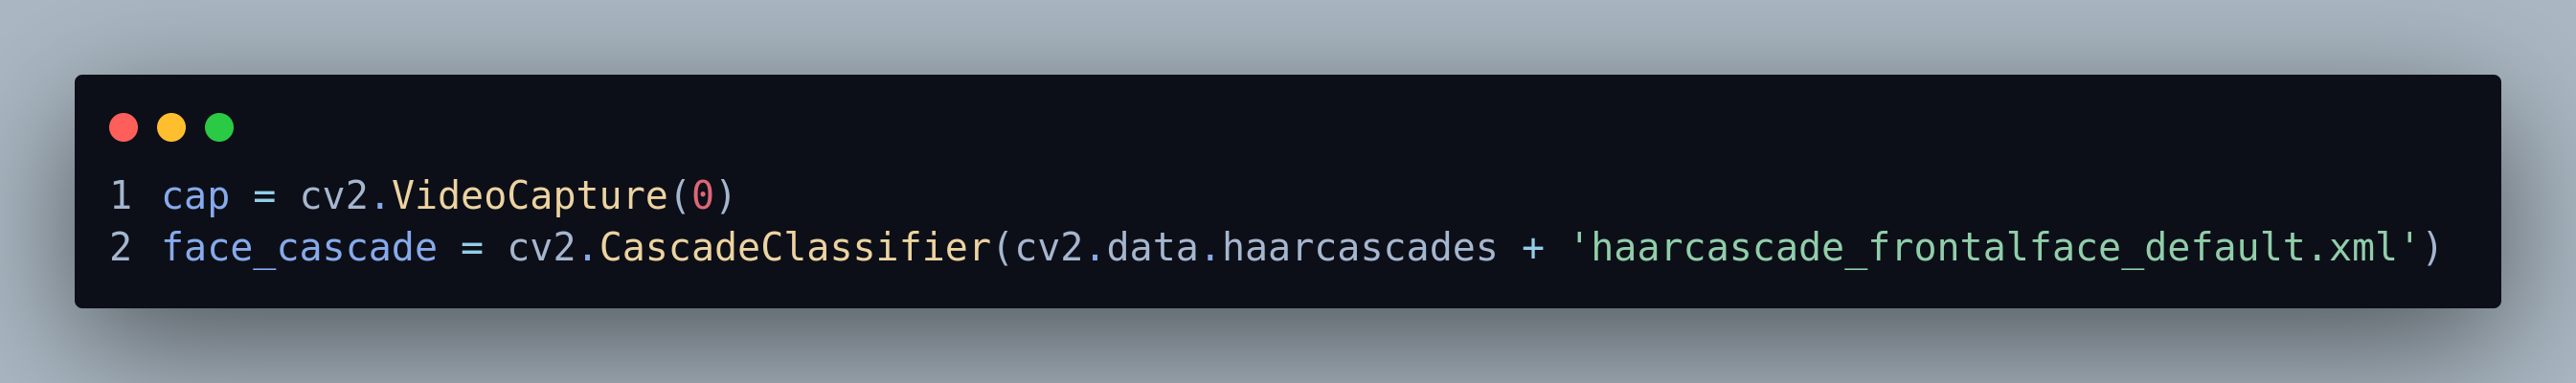
\includegraphics[width=1.0\linewidth]{imagenes/des23.png}
    \caption{Ingresar caption}
    \label{fig:enter-label}
\end{figure}

Iniciamos un bucle para capturar los frames y convertirlo a escala de grises. Los rostros detectados se almacenan en la variable faces como una lista de coordenadas (x, y, w, h) que representan la posición y el tamaño de cada rostro detectado.

\begin{figure}[h]
    \centering
    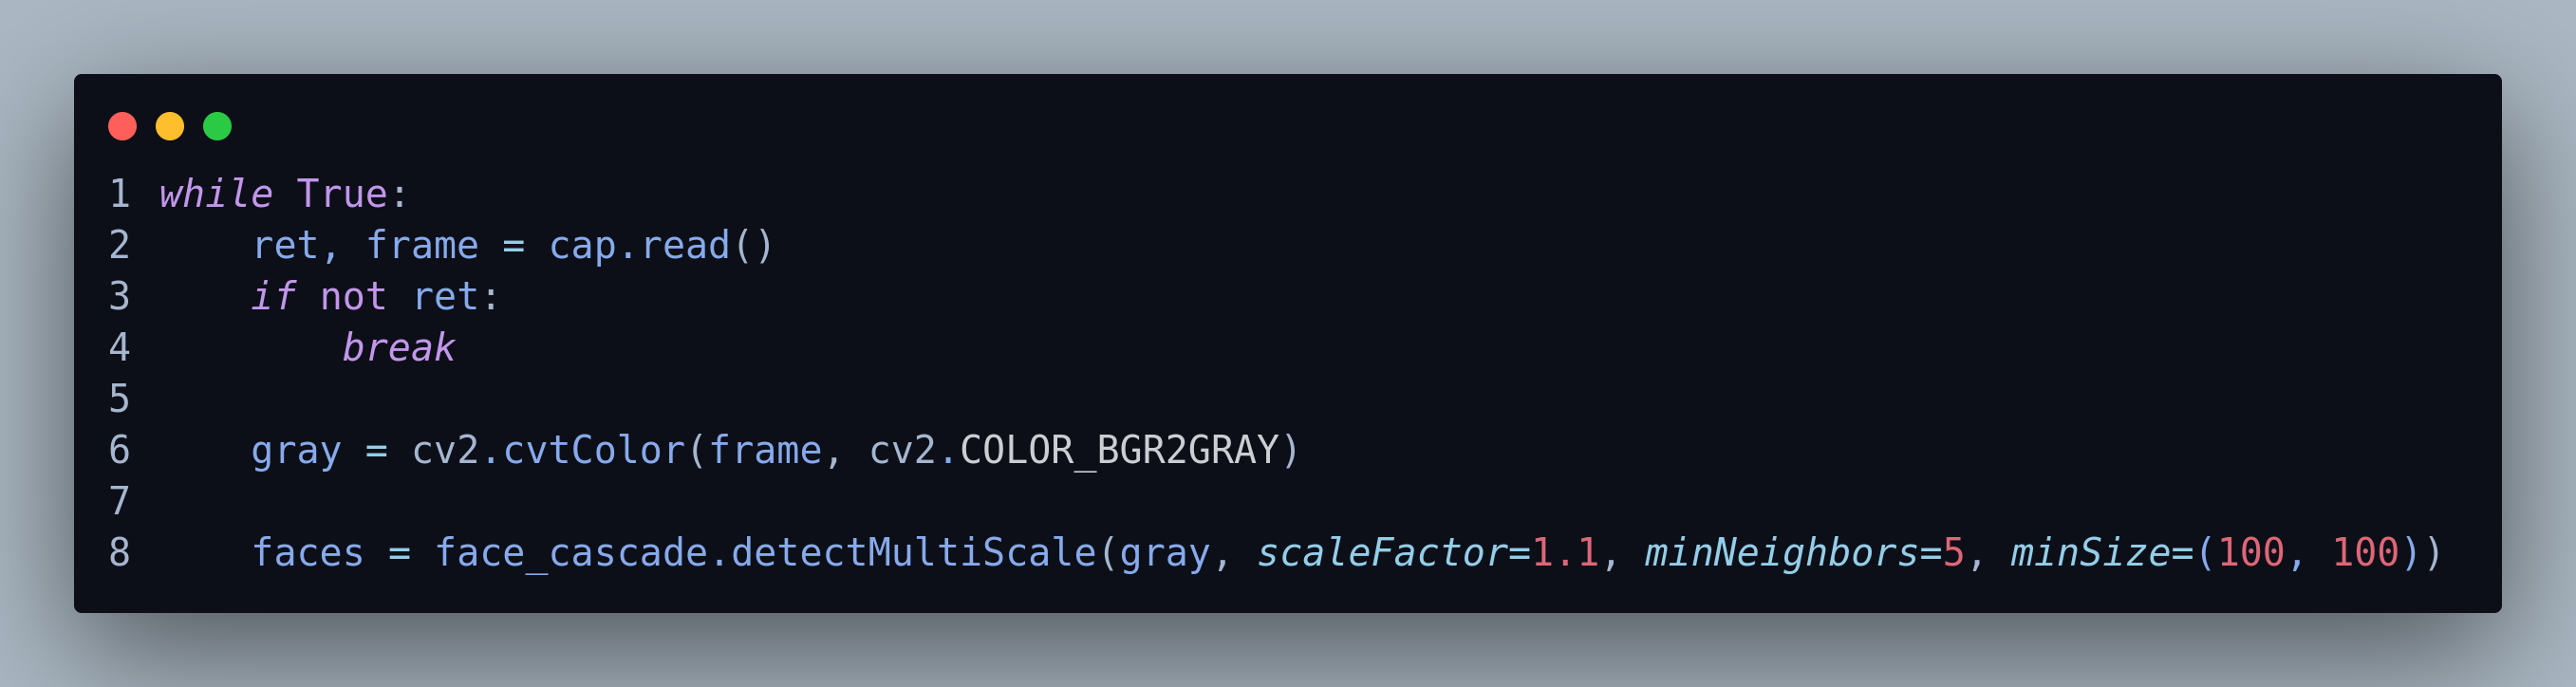
\includegraphics[width=1.0\linewidth]{imagenes/des24.png}
    \caption{Ingresar caption}
    \label{fig:enter-label}
\end{figure}

Se itera sobre cada rostro detectado en la lista faces.

\begin{itemize}
    {\bfseries\item gray[y:y+h, x:x+w]:} Extrae la región de interés (ROI) del rostro en la imagen en escala de grises .Esto selecciona solo la parte de la imagen que contiene el rostro detectado.
    {\bfseries\item cv2.resize(roi\_gray, (200, 200)):} Redimensiona la ROI a un tamaño fijo de 200x200 píxeles, esto es necesario porque el modelo de reconocimiento facial espera imágenes de entrada con dimensiones específicas.
    {\bfseries\item label, confidence = model.predict(roi\_gray):} Utiliza el modelo de reconocimiento facial para predecir la identidad del rostro, label es el código asignado al rostro, confidence es un valor que indica la confianza de la predicción donde un valor más bajo indica mayor confianza.
    {\bfseries\item cv2.rectangle(frame, (x, y), (x+w, y+h), (255, 0, 0), 2):} Dibuja un rectángulo azul (color (255, 0, 0)) alrededor del rostro detectado en el fotograma original (frame).
\end{itemize}

\begin{figure}[h]
    \centering
    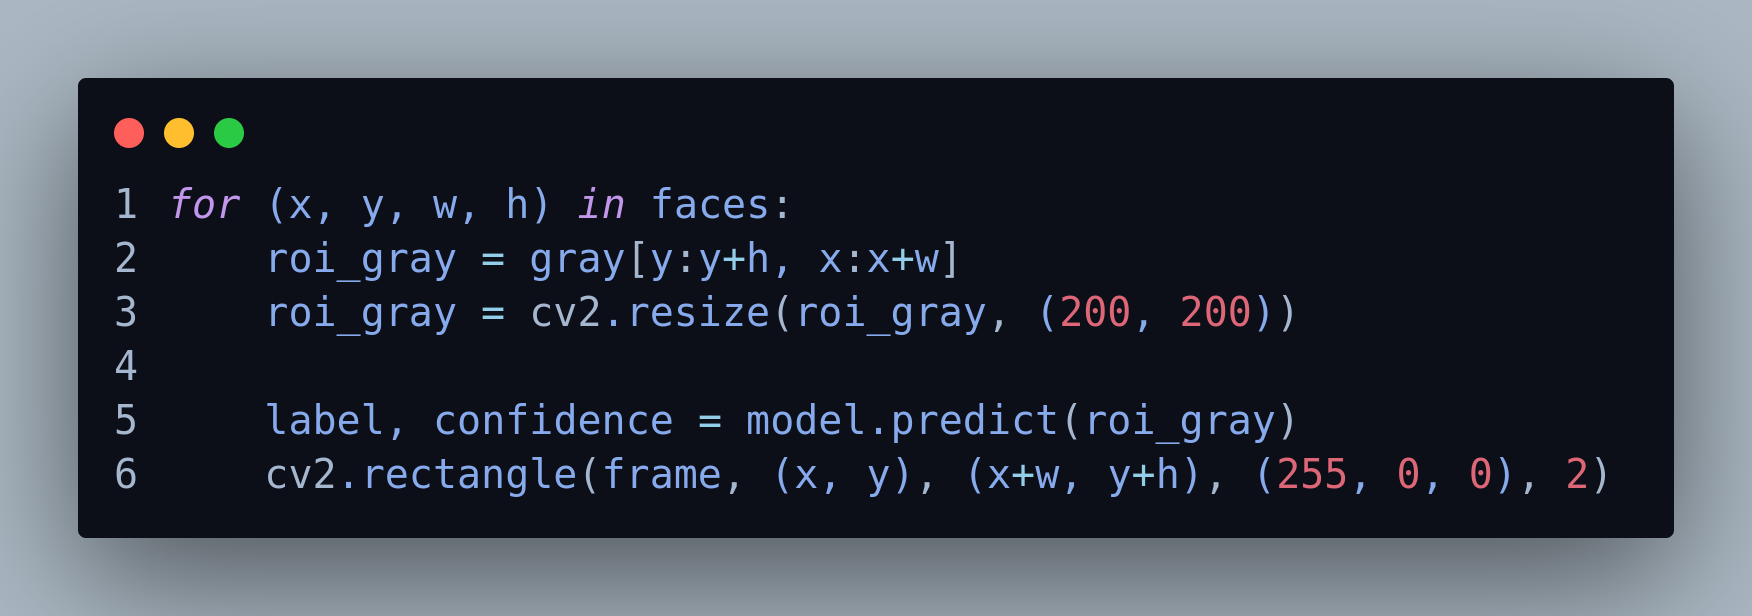
\includegraphics[width=0.9\linewidth]{imagenes/des25.png}
    \caption{Ingresar caption}
    \label{fig:enter-label}
\end{figure}

Si la confianza de la predicción es menor que un umbral (5500), se considera que el rostro ha sido reconocido.

\begin{itemize}
    {\bfseries\item cv2.putText:} Muestra texto sobre el fotograma para indicar el resultado de la predicción.
    {\bfseries\item cv2.imshow('Video', frame):} Muestra el fotograma procesado en una ventana llamada "Video", con los rectángulos y etiquetas superpuestos.
\end{itemize}

\begin{figure}[h]
    \centering
    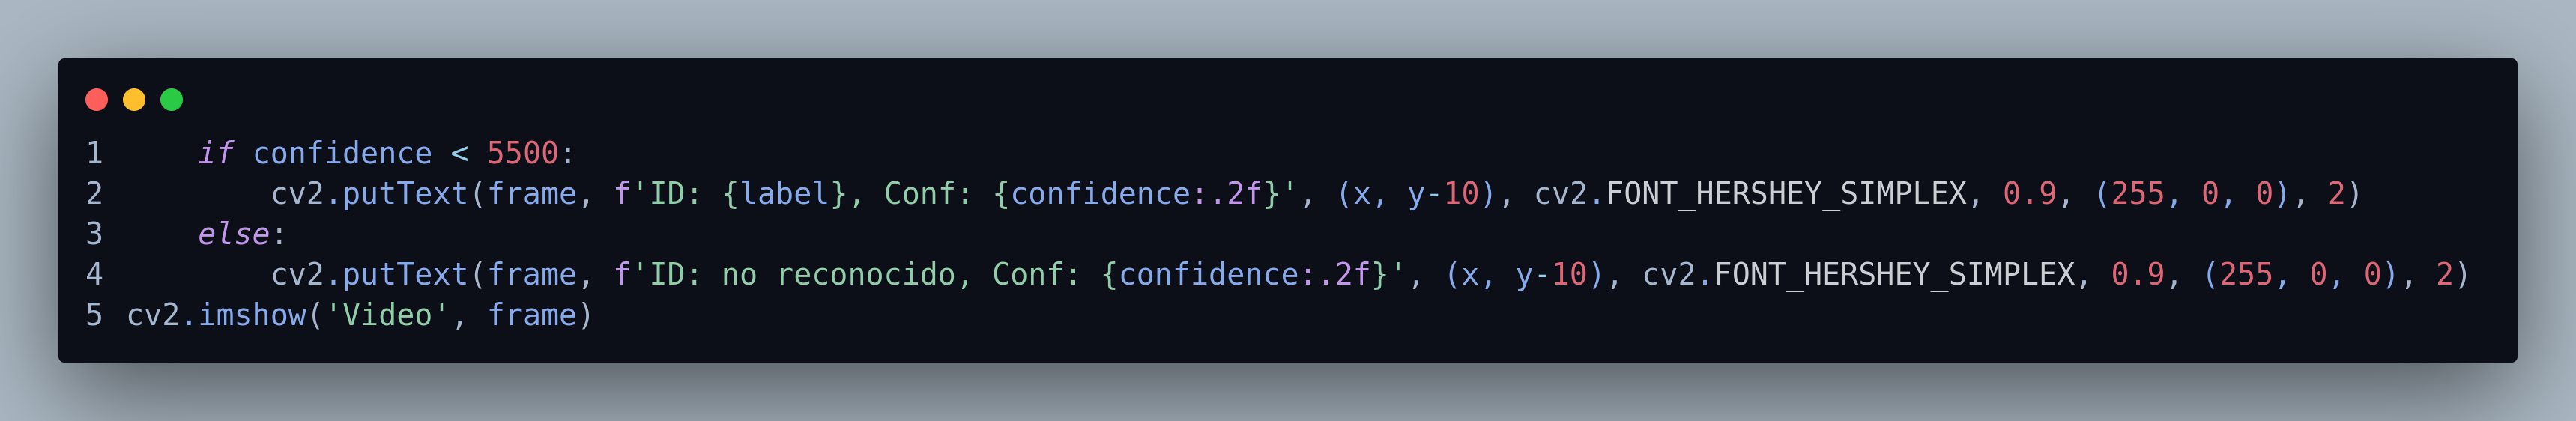
\includegraphics[width=1.0\linewidth]{imagenes/des26.png}
    \caption{Ingresar caption}
    \label{fig:enter-label}
\end{figure}

Si se presiona la tecla 'q' la función finaliza y se detiene la captura de video.  Luego, libera los recursos de la cámara y cierra las ventanas de OpenCV para garantizar un cierre limpio del programa.

\begin{figure}[h]
    \centering
    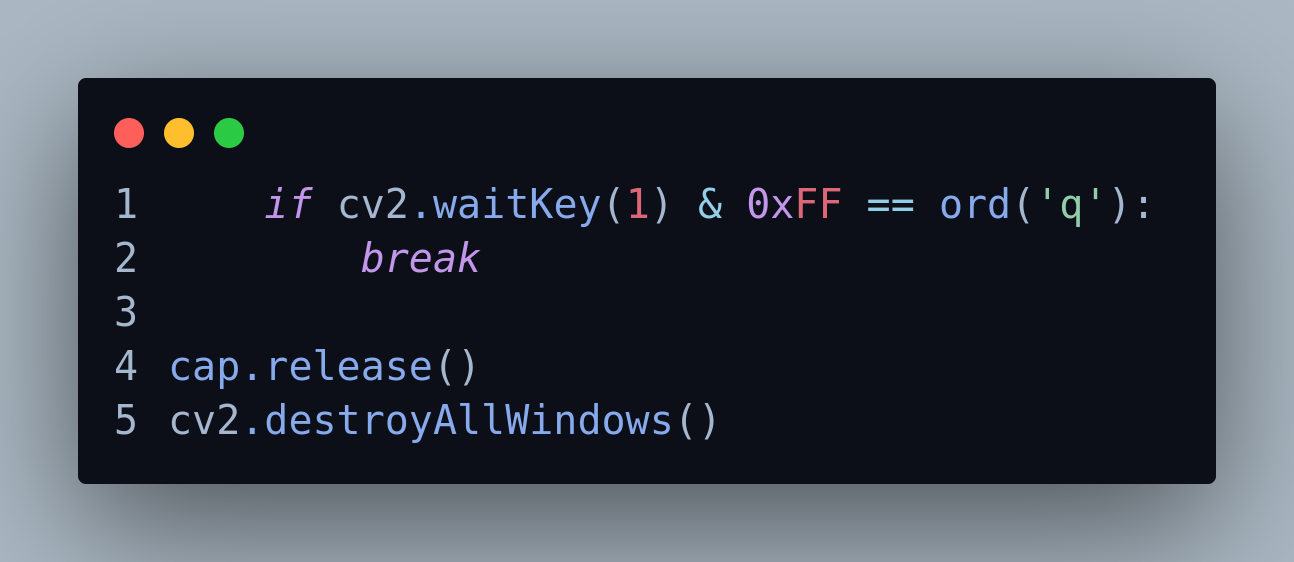
\includegraphics[width=0.75\linewidth]{imagenes/des27.png}
    \caption{Caption}
    \label{fig:enter-label}
\end{figure}


%Resultados
\section{Resultados}
\subsection{Ejemplo}


%Conclusiones y recomendaciones
\section{Conclusiones}
El desarrollo del sistema de reconocimiento facial permite alcanzar satisfactoriamente los objetivos planteados. Se logró implementar un programa funcional que realiza la detección de rostros en tiempo real, empleando las técnicas de visión por computadora y machine learning. Esta implementación propone reemplazar el método actual de identificación el cual se basa en el uso de carnet físicos. Siendo que este cambio propone una alternativa moderna, segura y automática.

El sistema demostró cierta versatilidad al ofrecer dos opciones para la recolección de los datos, lo que facilita su uso en diferentes escenarios y contextos. Además la etapa de preprocesamiento mejoró la eficiencia computacional en gran medida así como también la precisión del modelo.

Uno de los fuertes de este proyecto fue que se incorporó una interfaz por consola que permitió a los usuarios hacer uso de este sistema con el manejo de un menú. Las pruebas realizadas en el entorno simulado confirmaron la capacidad del sistema para identificar de manera correcta a los usuarios, mostrando un nivel de confianza con cada persona que ayuda a reducir la probabilidad de posibles suplantadores.

Por último, el proyecto no solo demostró el avance en la automatización del control de accesos, sino también sentó las bases para futuras mejoras y ampliaciones dentro y fuera de la universidad. Además, afianzó y expandió las habilidades técnicas en programación con Python, haciendo uso de librerías como OpenCv y Pandas, y fundamentos de machine learning, así como el correcto uso de la plataforma colaborativa GitHub para su correcto desarrollo.


%Recomendaciones
\section{Recomendaciones}
Se recomienda sustituir el modelo Eigenfaces por el LBPH para mejorar la precisión del reconocimiento facial, especialmente en condiciones de iluminación variable y cuando se requiera procesar un mayor número de usuarios.

Asimismo, se sugiere integrar una base de datos centralizada que permita almacenar y consultar los registros de asistencia de forma estructurada y segura. Para aumentar la robustez del sistema sería beneficioso ampliar la variedad de muestras por usuario e implementar técnicas de aumento de datos que mejoren la generalización del modelo.

Además, se recomienda desarrollar una interfaz gráfica o una versión móvil, que facilite el uso del sistema en contextos reales por personal administrativo o técnico. Finalmente, se plantea evaluar el despliegue del sistema en otras facultades u organizaciones que enfrentan retos similares en el control de accesos.


%Anexos
\section{Anexos}
bbbbbbbbbbbbbbb

%Bibliografía
\bibliographystyle{apacite}
\bibliography{bibliografia.bib}

}
%Fin del cuerpo del documento
\end{document}